\documentclass[12pt,a4paper,openany]{report}

% -------------------- PACKAGES --------------------
\usepackage[a4paper,left=1.5in,right=1in,top=1in,bottom=1in]{geometry}
\usepackage[T1]{fontenc}
\usepackage{amsmath}
\usepackage{amssymb}
\usepackage{mathptmx}
\usepackage{graphicx}
\usepackage{fancyhdr}
\usepackage{setspace}
\usepackage{titlesec}
\usepackage{tocloft}
\usepackage{float}
\usepackage{array}
\usepackage{longtable}
\usepackage{xcolor}
\usepackage{caption}
\usepackage{microtype}
\usepackage{listings}
\usepackage{hyperref}
\hypersetup{hidelinks}
\emergencystretch=2em

% -------------------- FIGURE/TABLE NUMBERING (HYPHEN FORMAT) --------------------
\renewcommand{\thefigure}{\arabic{chapter}-\arabic{figure}}
\renewcommand{\thetable}{\arabic{chapter}-\arabic{table}}

% -------------------- LIST OF FIGURES / TABLES ENTRY FORMAT --------------------
% Prefix entries with "Figure"/"Table" and a colon, e.g. "Figure 4-1: ..."
\renewcommand{\cftfigpresnum}{Figure~}
\renewcommand{\cftfigaftersnum}{:}
\renewcommand{\cfttabpresnum}{Table~}
\renewcommand{\cfttabaftersnum}{:}
\setlength{\cftfignumwidth}{2.7cm}
\setlength{\cfttabnumwidth}{2.5cm}

% tocloft typesets the ToC/LoF/LoT titles itself (bypassing titlesec's \chapter*),
% and its default title font is \Huge\bfseries. Match the 12pt bold chapter style
% so these titles look identical to the manual \chapter*{LIST OF ABBREVIATIONS}.
\renewcommand{\cfttoctitlefont}{\normalfont\bfseries\fontsize{12}{14}\selectfont}
\renewcommand{\cftloftitlefont}{\normalfont\bfseries\fontsize{12}{14}\selectfont}
\renewcommand{\cftlottitlefont}{\normalfont\bfseries\fontsize{12}{14}\selectfont}
\setlength{\cftbeforetoctitleskip}{0pt}
\setlength{\cftaftertoctitleskip}{12pt}
\setlength{\cftbeforeloftitleskip}{0pt}
\setlength{\cftafterloftitleskip}{12pt}
\setlength{\cftbeforelottitleskip}{0pt}
\setlength{\cftafterlottitleskip}{12pt}

% -------------------- CAPTION SETUP --------------------
\captionsetup{%
  justification=centering,
  font={small, bf},
  labelsep=space,      % space after "Figure 4-1"
  singlelinecheck=false
}

% -------------------- CODE LISTING STYLE --------------------
\definecolor{codebg}{gray}{0.96}
\definecolor{codekw}{RGB}{0,0,180}
\definecolor{codecomment}{RGB}{0,128,0}
\definecolor{codestr}{RGB}{163,21,21}
\definecolor{codeline}{gray}{0.5}
\lstdefinestyle{pystyle}{
	language=Python,
	basicstyle=\ttfamily\footnotesize,
	keywordstyle=\color{codekw}\bfseries,
	commentstyle=\color{codecomment}\itshape,
	stringstyle=\color{codestr},
	numbers=left,
	numberstyle=\tiny\color{codeline},
	numbersep=8pt,
	frame=single,
	rulecolor=\color{codeline},
	backgroundcolor=\color{codebg},
	showstringspaces=false,
	breaklines=true,
	breakatwhitespace=true,
	tabsize=4,
	captionpos=b,
	xleftmargin=14pt,
	xrightmargin=6pt,
	aboveskip=6pt,
	belowskip=6pt,
	literate={-}{-}1
}

% -------------------- LINE SPACING --------------------
\onehalfspacing

% Footer distance: 0.5 inch from bottom as required by template
\setlength{\footskip}{0.5in}

% Table captions appear above tables per template; figure captions remain below
\captionsetup[table]{position=top, font=small, labelfont=bf, labelsep=period}
\captionsetup[figure]{position=bottom, font=small, labelfont=bf, labelsep=period}

% -------------------- PAGE STYLE --------------------
\pagestyle{fancy}
\fancyhf{}
\cfoot{\thepage}
\renewcommand{\headrulewidth}{0pt}
\renewcommand{\footrulewidth}{0pt}
\setlength{\headheight}{15pt}

\fancypagestyle{plain}{%
	\fancyhf{}%
	\cfoot{\thepage}%
	\renewcommand{\headrulewidth}{0pt}%
}

\makeatletter
\let\ps@plain\ps@fancy
\makeatother

% -------------------- HEADING FORMATS --------------------
\titleformat{\chapter}[block]
	{\normalfont\bfseries\fontsize{12}{14}\selectfont}
	{\thechapter.}{0.8em}{\MakeUppercase}
\titlespacing*{\chapter}{0pt}{0pt}{12pt}

\titleformat{name=\chapter,numberless}[block]
	{\normalfont\bfseries\fontsize{12}{14}\selectfont}
	{}{0pt}{\MakeUppercase}
\titlespacing*{name=\chapter,numberless}{0pt}{0pt}{12pt}

\titleformat{\section}
	{\normalfont\bfseries\fontsize{12}{14}\selectfont}
	{\thesection.}{1em}{}
\titlespacing*{\section}{0pt}{0pt}{10pt}

\titleformat{\subsection}
	{\normalfont\bfseries\fontsize{12}{14}\selectfont}
	{\thesubsection.}{1em}{}
\titlespacing*{\subsection}{0pt}{0pt}{8pt}

% -------------------- TITLES --------------------
\renewcommand{\contentsname}{TABLE OF CONTENTS}
\renewcommand{\listfigurename}{LIST OF FIGURES}
\renewcommand{\listtablename}{LIST OF TABLES}
\renewcommand{\bibname}{REFERENCES}

% -------------------- DOCUMENT --------------------
\begin{document}
\sloppy

\pagenumbering{gobble}

% ============================================================================
% COVER PAGE
% ============================================================================
\begin{titlepage}
	\newgeometry{left=1in,right=1in,top=1in,bottom=1in}
	\thispagestyle{empty}
	\begin{center}
		\begin{spacing}{1.5}
			
\includegraphics[width=6.5cm]{tulogo.png}
			
			\vspace{8mm}
			\textbf{\MakeUppercase{TRIBHUVAN UNIVERSITY}}\\
			\textbf{\MakeUppercase{INSTITUTE OF ENGINEERING}}\\
			\textbf{\MakeUppercase{THAPATHALI CAMPUS}}
			
			\vfill
			\textbf{A PROJECT REPORT}\\
			\textbf{ON}
			\vspace{4mm}
			\textbf{\MakeUppercase{Multi-Agent Data Analysis and Insight Generation Platform for Financial and Sales Data}}
			
			\vfill
			\textbf{Submitted By:}\\
			Prashant Kafle (THA080BCT026)\\
			Roshan Poudel (THA080BCT036)\\
			Santosh Khadka (THA080BCT039)\\
			Sushil Bhatta (THA080BCT048)
			
			\vfill
			\textbf{Submitted To:}\\
			Department of Electronics and Computer Engineering\\
			Thapathali Campus\\
			Kathmandu, Nepal
			
			\vfill
			August, 2026
		\end{spacing}
	\end{center}
	\restoregeometry
\end{titlepage}

% ============================================================================
% TITLE PAGE (with supervisor and degree)
% ============================================================================
\begin{titlepage}
	\newgeometry{left=1in,right=1in,top=1in,bottom=1in}
	\thispagestyle{empty}
	\begin{center}
		\begin{spacing}{1.5}
			
\includegraphics[width=6.5cm]{tulogo.png}
			
			\vspace{8mm}
			\textbf{\MakeUppercase{TRIBHUVAN UNIVERSITY}}\\
			\textbf{\MakeUppercase{INSTITUTE OF ENGINEERING}}\\
			\textbf{\MakeUppercase{THAPATHALI CAMPUS}}
			
			\vfill
			\textbf{A PROJECT REPORT}\\
			\textbf{ON}
			\vspace{4mm}
			\textbf{\MakeUppercase{Multi-Agent Data Analysis and Insight Generation Platform for Financial and Sales Data}}
			
			\vfill
			\textbf{Submitted By:}\\
			Prashant Kafle (THA080BCT026)\\
			Roshan Poudel (THA080BCT036)\\
			Santosh Khadka (THA080BCT039)\\
			Sushil Bhatta (THA080BCT048)
			
			\vfill
			\textbf{Submitted To:}\\
			Department of Electronics and Computer Engineering\\
			Thapathali Campus\\
			Kathmandu, Nepal
			
			\vspace{4mm}
			In partial fulfillment for the award of the Bachelor's Degree in Computer Engineering.
			
			\vspace{4mm}
			\textbf{Under the Supervision of}\\
			Er. Rajad Shakya
			
			\vfill
			August, 2026
		\end{spacing}
	\end{center}
	\restoregeometry
\end{titlepage}

\clearpage
\pagenumbering{roman}
\setcounter{page}{1}

% --- DECLARATION ---
\chapter*{DECLARATION}
\addcontentsline{toc}{chapter}{DECLARATION}
\phantomsection

We hereby declare that the report of the project entitled \textbf{``Multi-Agent Data Analysis and Insight Generation Platform for Financial and Sales Data''} which is being submitted to the \textbf{Department of Electronics and Computer Engineering, IOE, Thapathali Campus}, in the partial fulfillment of the requirements for the award of the Degree of Bachelor of Engineering in \textbf{Computer Engineering}, is a bonafide report of the work carried out by us. The materials contained in this report have not been submitted to any University or Institution for the award of any degree and we are the only authors of this complete work and no sources other than the listed here have been used in this work.

\vspace{2em}
\noindent Prashant Kafle (THA080BCT026)\\
Roshan Poudel (THA080BCT036)\\
Santosh Khadka (THA080BCT039)\\
Sushil Bhatta (THA080BCT048)

\vspace{1em}
\noindent \textbf{Date:} August, 2026

\clearpage

% --- CERTIFICATE OF APPROVAL ---
\chapter*{CERTIFICATE OF APPROVAL}
\addcontentsline{toc}{chapter}{CERTIFICATE OF APPROVAL}
\phantomsection

The undersigned certify that they have read and recommended to the \textbf{Department of Electronics and Computer Engineering, IOE, Thapathali Campus}, a project work entitled \textbf{``Multi-Agent Data Analysis and Insight Generation Platform for Financial and Sales Data''} submitted by \textbf{Prashant Kafle (THA080BCT026), Roshan Poudel (THA080BCT036), Santosh Khadka (THA080BCT039), and Sushil Bhatta (THA080BCT048)} in partial fulfillment for the award of Bachelor's Degree in \textbf{Computer Engineering}. The Project was carried out under special supervision and within the time frame prescribed by the syllabus.

We found the students to be hardworking, skilled and ready to undertake any related work to their field of study and hence we recommend the award of partial fulfillment of Bachelor's degree of Computer Engineering.

\vspace{2em}
\noindent Project Supervisor\\
Er. Rajad Shakya\\
Department of Electronics and Computer Engineering, Thapathali Campus

\vspace{1em}
\noindent External Examiner\\
\rule{5cm}{0.4pt}

\vspace{1em}
\noindent Project Co-ordinator\\
Asst. Prof. Anup Shrestha\\
Department of Electronics and Computer Engineering, Thapathali Campus

\vspace{1em}
\noindent Head of the Department\\
\rule{5cm}{0.4pt}\\
Department of Electronics and Computer Engineering, Thapathali Campus

\vspace{1em}
\noindent August, 2026

\clearpage

% --- COPYRIGHT ---
\chapter*{COPYRIGHT}
\addcontentsline{toc}{chapter}{COPYRIGHT}
\phantomsection

The author has agreed that the library, Department of Electronics and Computer Engineering, Thapathali Campus, may make this report freely available for inspection. Moreover, the author has agreed that the permission for extensive copying of this project work for scholarly purpose may be granted by the professor/lecturer, who supervised the project work recorded herein or, in their absence, by the head of the department. It is understood that the recognition will be given to the author of this report and to the Department of Electronics and Computer Engineering, IOE, Thapathali Campus in any use of the material of this report. Copying of publication or other use of this report for financial gain without approval of the Department of Electronics and Computer Engineering, IOE, Thapathali Campus and author's written permission is prohibited.

Request for permission to copy or to make any use of the material in this project in whole or part should be addressed to department of Electronics and Computer Engineering, IOE, Thapathali Campus.

\clearpage

% --- ACKNOWLEDGEMENT ---
\chapter*{ACKNOWLEDGEMENT}
\addcontentsline{toc}{chapter}{ACKNOWLEDGEMENT}
\phantomsection

\begin{small}
We would like to express our sincere gratitude to the Department of Electronics and Computer Engineering, Thapathali Campus, Institute of Engineering, Tribhuvan University, for providing us the opportunity to work on this project.

We are deeply indebted to our supervisor, Er. Rajad Shakya, for his guidance, constructive feedback, and continuous encouragement throughout the development of this project. His suggestions have helped us refine both the technical design and the report structure.

We also thank the faculty members of the department for creating an academic environment that supports practical engineering work. Finally, we are grateful to our friends and families for their patience and support during this phase of the project.

\vspace{2em}
\noindent\textbf{Submitted By:}\\
Prashant Kafle (THA080BCT026)\\
Roshan Poudel (THA080BCT036)\\
Santosh Khadka (THA080BCT039)\\
Sushil Bhatta (THA080BCT048)

\vspace{1em}
\hfill August, 2026
\end{small}

\clearpage

% --- ABSTRACT ---
\chapter*{ABSTRACT}
\addcontentsline{toc}{chapter}{ABSTRACT}
\phantomsection

\begin{small}
This project presents a complete end-to-end multi-agent system that transforms raw CSV-based financial and sales data into validated, professionally formatted analytical reports with interactive charts and grounded plain-language insights. The system is built around a LangGraph pipeline of six specialized agents: structural profiling, semantic tagging, context-aware preprocessing, statistical analysis and visualization, deterministic output validation with a Cohen's kappa gate, and hybrid report generation with claim grounding. A FastAPI backend provides secure file uploads, job management with PostgreSQL persistence, and Server-Sent Events (SSE) for live progress streaming. A React 19 frontend offers a no-code web interface for uploading datasets, monitoring agent execution, viewing interactive charts, downloading HTML/PDF reports, and querying data via a retrieval-augmented generation (RAG) chat. The system is dataset-agnostic, accepting arbitrary tabular CSV files of financial and sales data; as a representative demonstration, a sample sales dataset is processed end-to-end through all six agents to produce a comprehensive report with KPI summaries, correlation matrices, trend analyses, anomaly detection, and validated findings. The system achieves end-to-end automation while maintaining auditability through logged transformations, confidence propagation, and rigorous validation checks, including Tier-1 contract enforcement and LLM--heuristic agreement scoring. This work demonstrates that agentic orchestration, combined with deterministic data processing and controlled LLM reasoning, can deliver reliable, accessible, and automated data analysis for small to medium organizations.
\end{small}

\vspace{1em}
\noindent\textbf{Keywords:} agentic frameworks, Cohen's kappa, FastAPI, financial analytics, LangGraph, multi-agent systems, RAG, React, reporting, sales analytics, validation

\clearpage

% --- TABLE OF CONTENTS (single spacing) ---
\begin{singlespace}
\tableofcontents
\end{singlespace}

\clearpage
\phantomsection
\addcontentsline{toc}{chapter}{LIST OF FIGURES}
\begin{singlespace}
\listoffigures
\end{singlespace}

\clearpage
\phantomsection
\addcontentsline{toc}{chapter}{LIST OF TABLES}
\begin{singlespace}
\listoftables
\end{singlespace}

\chapter*{LIST OF ABBREVIATIONS}
\addcontentsline{toc}{chapter}{LIST OF ABBREVIATIONS}
\phantomsection

\renewcommand{\arraystretch}{1.2}
\begin{longtable}{p{3cm} p{9cm}}
\textbf{AI} & Artificial Intelligence \\
\textbf{API} & Application Programming Interface \\
\textbf{BI} & Business Intelligence \\
\textbf{CORS} & Cross-Origin Resource Sharing \\
\textbf{CSV} & Comma-Separated Values \\
\textbf{DAG} & Directed Acyclic Graph \\
\textbf{DOECE} & Department of Electronics and Computer Engineering \\
\textbf{ECharts} & Enterprise Charts \\
\textbf{GQA} & Grouped-Query Attention \\
\textbf{IOE} & Institute of Engineering \\
\textbf{IQR} & Interquartile Range \\
\textbf{JSON} & JavaScript Object Notation \\
\textbf{JWT} & JSON Web Token \\
\textbf{KS} & Kolmogorov–Smirnov \\
\textbf{KV} & Key-Value (cache) \\
\textbf{LLM} & Large Language Model \\
\textbf{LPU} & Language Processing Unit \\
\textbf{MAD} & Median Absolute Deviation \\
\textbf{MAPE} & Mean Absolute Percentage Error \\
\textbf{MoM} & Month-over-Month \\
\textbf{OLS} & Ordinary Least Squares \\
\textbf{ORM} & Object-Relational Mapping \\
\textbf{PDF} & Portable Document Format \\
\textbf{QoQ} & Quarter-over-Quarter \\
\textbf{RAG} & Retrieval-Augmented Generation \\
\textbf{REST} & Representational State Transfer \\
\textbf{SSE} & Server-Sent Events \\
\textbf{TU} & Tribhuvan University \\
\textbf{UUID} & Universally Unique Identifier \\
\end{longtable}

\clearpage
\pagenumbering{arabic}

\chapter{INTRODUCTION}

\section{Background}

Data-driven decision-making has become a foundational requirement for organizational effectiveness in health, agriculture, education, and commerce. In Nepal, the government's Digital Nepal Framework explicitly prioritizes data-centric governance across these sectors. However, the operational reality for most organizations particularly those outside the Kathmandu Valley remains characterized by manual spreadsheet management and underutilized datasets. The technical barrier to entry for modern analytics is high: tools demand proficiency in query languages, schema design, or statistical software, while enterprise platforms carry licensing costs that are unsustainable for donor-funded non-governmental organizations (NGOs) and municipal bodies. The emergence of LLMs and agentic orchestration frameworks has created a new design space for autonomous software systems \cite{dwivedi2023}. LLMs can now interpret column semantics and narrate statistical findings in natural language, while agentic frameworks such as LangGraph enable reliable, stateful, multi-step automation. The convergence of these technologies makes it feasible to build a pipeline that replicates the workflow of a human data analyst validation, cleaning, profiling, visualization, statistical testing, interpretation, and reporting without requiring human intervention at each step.

\section{Motivation}

The motivation for this project is based on the following points:

\begin{itemize}
	\item Despite the availability of data, many organizations lack the technical expertise required to analyze and interpret it effectively.
	\item Traditional data analysis tools often require statistical knowledge, programming skills, or manual report interpretation.
	\item Existing AI-based systems using LLMs may generate unverified or hallucinated insights, leading to unreliable conclusions.
	\item Recent advances in Artificial Intelligence and Multi-Agent Systems provide an opportunity to automate complex analytical tasks.
\end{itemize}

\section{Problem Definition}

Organizations accumulate data daily sales records, transaction logs, expense sheets, customer information yet cannot efficiently convert this data into insights that drive strategy and decision-making.

Existing challenges:

\begin{enumerate}
	\item \textbf{Manual workflows:} Data analysis currently requires skilled staff to manually clean data, calculate metrics, build charts, and compile reports a process taking days to weeks

	\item \textbf{Lack of standardization:} Without a systematic methodology, different people produce inconsistent results, making it difficult to compare periods or validate findings

	\item \textbf{Limited accessibility:} Analytics tools require specialized knowledge. Non-technical stakeholders cannot ask ad-hoc questions without analyst intermediaries

\end{enumerate}

This project proposes an end-to-end automated system that takes raw sales and financial CSV data and produces validated, auditable, professionally formatted reports with trend insights and recommendations.

\section{Objectives}

The primary objectives of this project are:

\begin{enumerate}
	\item Develop an autonomous multi-agent system that converts raw sales and financial data (CSV format) into professional analytical reports and forecasts without manual coding

	\item Democratize basic financial analytics and sales optimization for small to medium businesses and organizations through a no-code web interface
\end{enumerate}

\section{Scope and Applications}

\hspace*{\parindent}\textbf{Technical Scope:}

\begin{itemize}
	\item Supports common business data types: sales records, transaction logs, expense sheets, in CSV format (with additional Excel loader path available)
	\item A complete six-agent pipeline (profiling, semantic tagging, preprocessing, statistical analysis, validation, and report generation) is implemented end-to-end
	\item Runs as a web application with FastAPI backend and React frontend, without requiring users to download additional software
\end{itemize}

\textbf{Primary Use Cases:}

\begin{enumerate}
	\item \textbf{Sales Performance Tracking:} Automated analysis of sales data to identify trends, top-performing products, seasonal patterns, and revenue forecasts for planning

	\item \textbf{Financial Reporting \& Budgeting:} Generation of expense summaries, income vs. expenditure analysis, budget tracking, and monthly/quarterly financial reports for small to medium organizations

	\item \textbf{Retail \& E-commerce Analytics:} Customer purchase behavior, inventory turnover analysis, demand forecasting, and sales channel comparison

	\item \textbf{Small Business Operations:} Cash flow trends, profit margin analysis, supplier/payment tracking, and operational dashboards without requiring accounting software expertise

	\item \textbf{Financial Data for Non-Finance Teams:} Simplified reports that translate raw financial/sales data into plain-language insights for managers, project leads, and decision-makers
\end{enumerate}

\section{Report Organization}

The remainder of this report is organized as follows. Chapter 2 reviews existing literature on traditional BI platforms, AI-assisted analytics, automated visualization, multi-agent frameworks, and positions the project within the research gap. Chapter 3 presents the requirement analysis, including functional and non-functional requirements, feasibility study, dataset analysis, and the current implementation status. Chapter 4 describes the theoretical approach, focusing on the Qwen3-27B language model and its architecture. Chapter 5 explains the overall system architecture, including the LangGraph pipeline, shared state, reliability propagation, backend services, and frontend workflow. Chapter 6 provides detailed implementation descriptions for each of the six agents, the FastAPI backend, and the React frontend. Chapter 7 presents the results and analysis from a complete run on the sample dataset, with tables, charts, and validation metrics. Chapter 8 discusses future enhancements and potential extensions. Chapter 9 concludes the report with a summary of contributions and achievements. Finally, the appendices provide additional technical details, cost estimates, timeline, and sample outputs.

\chapter{LITERATURE REVIEW}

\section{Traditional Data Analytics Platforms}
Platforms for Business Intelligence like Microsoft Power BI, Tableau, and Google Looker Studio are popular choices when it comes to data visualization, creation of dashboards, and decision making. These technologies offer a variety of data connectivity options, visualization functions, and reporting features, helping companies track their key performance indicators and business processes. With all their ecosystem and integration possibilities, these BI systems can be used by large corporations. However, there is a number of disadvantages of BI systems as well. First of all, users need to know database schema, configure their dashboards, and prepare the data themselves. Moreover, licensing and other infrastructure expenses may prove to be expensive for small companies, educational institutions, and non-profit organizations lacking funds. However, one of the major drawbacks of traditional BI systems is their lack of automation in interpretation, relying only on visualization.
According to Dwivedi et al. \cite{dwivedi2023}, large language models are changing data analytics. LLMs let us interact naturally, reason automatically, and get smart decision support. The authors argue that we need to progress from static dashboards to AI systems that offer insightful auto-recommendations. This points out an important research gap. To address it, we should develop intelligent, multi-agent data analyst systems.

\section{AI-Assisted Analytics and Large Language Model-Based Data Analysis}
LLMs are changing data analytics with their ability to chat naturally about data \cite{dwivedi2023}. Tools like ChatGPT with Code Interpreter and other assistant-style systems let people upload datasets and get back code, charts, stats analyses, and plain text explanations \cite{openai2024}. This is big because it makes data analysis easier for those without a ton of technical skills.

One huge plus is how easy these platforms are to use. Regular folks can talk to a dataset without needing loads of coding knowledge. Researchers show that LLMs can handle lots of jobs, like cleaning data, doing exploratory analysis, spitting out visuals, and even putting together reports \cite{sun2024}.

Still, there are some downsides. For one, getting the same result each time is tricky since outcomes rely heavily on the questions you ask. You might phrase things differently and end up with entirely distinct findings. Also, these systems tend to be single agent setups that don’t follow a strict workflow or include checks for accuracy. There’s no built-in QA process, and sometimes the code generated can have errors or missing steps \cite{liu2023chatgpt, maynez2020faithfulness}. This really drives the need for more complex systems that employ different agents for doing analysis, verifying results, and generating reports. Recent work on retrieval-augmented generation (RAG) has shown promise in grounding LLM responses in external knowledge bases, reducing hallucinations and improving factual accuracy \cite{lewis2020rag}. This approach is particularly relevant for the dataset chat and claim-grounding features implemented in this project.

\section{Automated Data Visualization from Tabular/CSV Data}
Several studies have investigated automated visualization generation from structured datasets. Data2Vis \cite{dibia2019} proposed a sequence-to-sequence neural architecture that translates datasets into Vega-Lite visualization specifications. VizML \cite{hu2019} applied machine learning to learn visualization design choices from over one million dataset-visualization pairs. Draco \cite{moritz2018} formalized visualization design knowledge as logical constraints to recommend effective visual encodings. DeepEye \cite{luo2018} further automated chart generation and ranking. These studies collectively demonstrate the feasibility of automated visualization generation and provide strong theoretical support for the Visualization Agent proposed in this research.

The main insight from this line of work is that visualization creation can be treated as a recommendation or generation task rather than a purely manual design task. This is especially relevant for CSV-based analysis workflows, where the system must decide whether to use bar charts, line charts, scatter plots, or other encodings based on the structure and semantics of the tabular data. The proposed project adopts this idea by using an agent that converts cleaned tabular outputs into appropriate static visualizations for reports.

\section{Agentic AI Frameworks and Multi-Agent Systems}
The newest stuff in Agentic AI includes LangGraph, CrewAI, and AutoGen frameworks that help different AI agents work together on big projects \cite{langchain2024, wu2023}. Traditionally, one AI does all the work, but these new setups let multiple agents take on tasks based on what they’re best at.

LangGraph helps manage agent teamwork with things like conditional routing and checkpointing. Meanwhile, AutoGen is all about letting agents chat back and forth, and CrewAI handles task delegation based on roles. Altogether, these tools show promise for building really smart, self-reliant systems that can figure out tough problems, plan, and coordinate tasks efficiently.

According to Wu et al. \cite{wu2023}, when you set up proper structures for AI conversations, teams of specialized agents can ace complex assignments. This covers everything from coding and math to answering questions and making decisions. It’s clear that such collaborations do better than lone agents.

Still, most work right now only applies these frameworks to areas like software engineering, web searches, Q\&A, and general reasoning. Not many have looked into how well they fit into fixed data analysis processes that mix deterministic stats ops with more uncertain language-model thinking. This gap presents an opportunity for the development of multi-agent systems specifically designed for automated data analysis and business intelligence workflows.

\section{Existing Research on Automated Data Analysis Systems}
Researchers are looking into artificial intelligence to make data analytics easier. They’re mixing machine learning, big language models, and natural language processing to help with exploring data, making it visual, and getting insights.

Sun et al. came up with LAMBDA, a Large Model Based Data Agent, which uses special AI agents to do data analysis \cite{sun2024}. These agents follow instructions in regular language to do tasks like code generation, stats, and visualizations. The cool thing is, when these agents work together, they improve accuracy and dependability more than solo agents \cite{sun2024}.

While there's been progress, most systems now only cover certain parts of the analytics job. For instance, statistical tools are great but aren’t very user-friendly, and some language model tools don’t always deliver consistent results because they rely too much on how you write prompts. Also, many current tools work in isolation they don’t all come together to form that full analytics process which would include everything from pre-processing data to generating reports.

So, we need a better way. There’s a call for a complete multi-agent setup that provides reliable and repeatable data analytics. This could revolutionize how we handle big data tasks.

\section{Research Gap and Project Positioning}
According to the literature reviewed, there is a lack of studies dedicated to multi-agent data processing systems that combine deterministic analytical algorithms with LLM-based reasoning in a reliable end-to-end analytics pipeline \cite{sun2024, wu2023}. Traditional BI tools require significant user involvement and technical expertise \cite{dwivedi2023}. While LLM-based systems improve accessibility, they do not inherently guarantee reproducibility, auditability, and structured execution workflows \cite{liu2023chatgpt, maynez2020faithfulness}. Multi-agent frameworks provide orchestration capabilities but have primarily been applied to software engineering and general reasoning tasks rather than autonomous data analytics and reporting \cite{wu2023, langchain2024}.
Therefore, this project proposes a LangGraph-based multi-agent analytics system in which specialized agents perform data ingestion, preprocessing, analysis, visualization, validation, and report generation. Deterministic analytical methods will be used for statistical computations, while an LLM-based agent will generate insights and explanations. The proposed system aims to improve reproducibility, accessibility, and automation of data analytics workflows for educational institutions, small businesses, and non-technical users.

\chapter{REQUIREMENT ANALYSIS}

\section{Functional Requirements}
\begin{itemize}
		\item Upload or load a structured dataset.
		\item Profile the dataset structure and missingness.
		\item Infer semantic metadata for columns.
		\item Preprocess and clean the data.
		\item Generate statistical summaries and visualizations.
		\item Validate the outputs before final reporting.
		\item Produce a final executive report.
\end{itemize}

\section{Non-Functional Requirements}
\begin{itemize}
		\item Reproducible execution through shared state and deterministic processing.
		\item Extensible agent-based design.
		\item Graceful handling of missing data, invalid input, and validation failures.
		\item Clear audit trail for preprocessing and validation decisions.
\end{itemize}

The most important non-functional requirement is traceability. The system does not hide intermediate decisions inside a black box; instead, it keeps outputs in the shared state and logs important actions as the pipeline proceeds. A second important requirement is robustness, because a report-generating system is only useful if it can continue operating sensibly when some inputs are incomplete or imperfect.

\section{Software Requirements}
The system is built on a modern Python-based backend with a React frontend. Key software components include:

\begin{itemize}
	\item \textbf{Python 3.12+}: Core programming language for the backend and agents.
	\item \textbf{FastAPI}: Web framework for REST API endpoints and SSE streaming.
	\item \textbf{LangGraph}: Orchestration framework for building the six-agent pipeline with conditional routing.
	\item \textbf{Pandas, NumPy, SciPy, Scikit-learn}: Data manipulation, statistical analysis, and machine learning utilities.
	\item \textbf{Matplotlib, ECharts}: Static and interactive chart generation.
	\item \textbf{Jinja2, WeasyPrint}: HTML templating and PDF rendering.
	\item \textbf{PostgreSQL with pgvector}: Optional persistent storage for job data and RAG embeddings.
	\item \textbf{React 19, Vite, TailwindCSS}: Frontend framework, build tool, and styling.
\end{itemize}

\section{Feasibility Study}

\subsection{Technical Feasibility}
The project leverages mature open-source libraries and cloud-based LLM APIs. Python's rich ecosystem for data processing (Pandas, Scikit-learn) and orchestration (LangGraph) provides a solid technical foundation. The use of Groq and Gemini APIs eliminates the need for expensive on-premise GPU infrastructure, making the system deployable on standard cloud VMs or even local machines with internet access. The React-based frontend ensures cross-platform compatibility.

\subsection{Operational Feasibility}
The no-code web interface significantly lowers the barrier to entry. Users can upload a CSV file and receive a complete analytical report without any programming or statistical expertise. The system is designed to be self-service, reducing dependency on specialized data analysts and accelerating decision-making cycles.

\subsection{Economic Feasibility}
The project's primary costs are variable LLM API usage fees. However, the deterministic fallback mechanisms and heuristic-based tagging reduce reliance on the LLM for every operation. The open-source nature of the core stack (Python, FastAPI, React, PostgreSQL) means no licensing fees. For small to medium organizations, the cost of API usage is negligible compared to the labor cost of manual data analysis.

\section{Dataset Analysis}
The system is designed to be dataset-agnostic and accepts arbitrary tabular CSV files of financial and sales data. For validation and demonstration, a representative sample dataset, \texttt{10000 Sales Records.csv}, is included in the project repository. This sample contains 10,000 rows and 14 columns, representing simulated global sales transactions. Its columns are:

\begin{itemize}
	\item \texttt{Region}, \texttt{Country}: Geographic fields (categorical).
	\item \texttt{Item Type}, \texttt{Sales Channel}, \texttt{Order Priority}: Categorical labels (12, 2, and 4 distinct values respectively).
	\item \texttt{Order Date}, \texttt{Ship Date}: Transaction and shipment dates (datetime).
	\item \texttt{Order ID}: Unique transaction identifier.
	\item \texttt{Units Sold}: Quantity sold (count).
	\item \texttt{Unit Price}, \texttt{Unit Cost}, \texttt{Total Revenue}, \texttt{Total Cost}, \texttt{Total Profit}: Monetary fields (currency).
\end{itemize}

The sample's mix of identifiers, dates, currencies, and categories makes it suitable for exercising the full pipeline. Agent 2's semantic tagging produces a blueprint in which \texttt{Order ID} is flagged as an identifier, \texttt{Order Date} and \texttt{Ship Date} as datetime, \texttt{Region} and \texttt{Country} as geographic, and the five monetary columns as currency. The preprocessing stage applies financial constraints, extracts date features, one-hot encodes categorical columns, and derives business metrics such as profit margin and revenue per unit.

\section{Requirement Status}
\begin{table}[H]
\centering
\caption{Implementation status of system requirements}
\label{tab:req-status}
\begin{tabular}{p{6cm} p{3cm} p{4cm}}
\hline
Requirement & Status & Notes \\
\hline
Data loading and profiling & Implemented & CSV-primary; Excel loader path exists \\
Semantic tagging & Implemented & Qwen3-27B with Gemini fallback \\
Preprocessing and cleaning & Implemented & Audit trail, quality scoring, KNN/iterative imputation \\
Statistics and charts & Implemented & ECharts + matplotlib, 10+ chart types \\
Validation gate & Implemented & Tier-1 contract checks + Cohen's kappa gate \\
Final report generation & Implemented & HTML/PDF via Jinja2/WeasyPrint \\
Backend API & Implemented & FastAPI + SSE + PostgreSQL/File storage \\
Frontend dashboard & Implemented & React 19 + Vite + TailwindCSS \\
Multi-format expansion & Partial & CSV-primary; JSON/Parquet not implemented \\
\hline
\end{tabular}
\end{table}

\chapter{THEORETICAL APPROACH}

The semantic tagging stage of this project relies on a Transformer-based Large Language Model (LLM) accessed through the Groq API, which serves the \texttt{qwen/qwen3.6-27b} model at high inference speed via purpose-built hardware. The system also includes an automatic Gemini fallback and a deterministic fallback for robustness. This chapter summarises only the concepts needed to understand how the model produces the JSON schema blueprint that drives preprocessing.

\section{Large Language Model Theory}

A Large Language Model is a neural network trained to model the probability distribution of natural language: given a sequence of previous tokens, it estimates the most likely next token. In this project the model is not used for free-form prose but as a structured reasoning component that reads column metadata and returns a strict JSON schema blueprint.

\subsection{Decoder-Only Transformer Architecture}
Earlier sequence models such as RNNs and LSTMs processed tokens one step at a time, which made training slow and long-range relationships hard to capture. The Transformer replaces recurrence with a self-attention mechanism that relates every token to every other token in parallel \cite{vaswani2017}. Text-generation models such as the Qwen family use a \emph{decoder-only} Transformer: a stack of identical blocks in which a causal mask allows the prediction at position $t$ to attend only to positions $1$ to $t$. This left-to-right constraint makes the model autoregressive, generating one token at a time.

\subsection{Tokenization and Embedding}
Raw text is first split into subword tokens, each mapped to an integer index in a fixed vocabulary of size $V$. Every index is then converted into a dense vector through a learned embedding matrix $E \in \mathbb{R}^{V \times d}$, where $d$ is the model dimension:
\begin{equation}
x = E(\text{token})
\label{eq:embed}
\end{equation}
Because self-attention is order-agnostic, a positional encoding is added to each embedding so the model can distinguish tokens by position as well as identity. In this project, the prompt containing column names, inferred types, and sample values is tokenized and embedded in exactly this way before inference.

\subsection{Self-Attention}
Self-attention lets each token gather information from other tokens. Three projections are formed from the input: queries $Q$, keys $K$, and values $V$, and they are combined using scaled dot-product attention:
\begin{equation}
\text{Attention}(Q,K,V) = \text{Softmax}\!\left(\frac{QK^{\top}}{\sqrt{d_k}}\right)V
\label{eq:attention}
\end{equation}
where $d_k$ is the key dimension and $\sqrt{d_k}$ scales the dot products to keep the softmax stable \cite{vaswani2017}. The Transformer runs several attention \emph{heads} in parallel so the model can capture different relationships at once. Each block also applies a position-wise feed-forward network with residual connections and layer normalization, which add capacity and keep the deep computation numerically stable.

\subsection{Next-Token Prediction}
After the final block, the last token representation is projected to a vector of logits $z$ of length $V$, which a softmax converts into a probability distribution over the vocabulary:
\begin{equation}
P(y_i) = \frac{\exp(z_i)}{\sum_j \exp(z_j)}
\label{eq:softmax}
\end{equation}
The model predicts the next token conditioned on all previous tokens and generates text autoregressively: each predicted token is appended to the sequence and fed back in to predict the following one, until a stopping condition is reached. A low sampling temperature is used in this project so the output is nearly deterministic, which is important because the response must be strictly valid JSON.

\begin{figure}[H]
\centering
\includegraphics[width=0.9\textwidth,height=0.82\textheight,keepaspectratio]{\detokenize{transformer_architecture.png}}
\caption{Decoder-only Transformer architecture used by modern LLMs}
\label{fig:transformer-architecture}
\end{figure}

\section{Groq API and LLM Inference Architecture}

The LLM backend of this system is the Groq API, which exposes the \texttt{qwen/qwen3.6-27b} model through an OpenAI-compatible REST interface. Groq achieves exceptionally low inference latency by running Transformer models on Language Processing Units (LPUs), custom silicon designed specifically for autoregressive token generation. The system also includes an automatic Gemini fallback (\texttt{gemini-flash-latest} and 3.x variants) and a deterministic fallback to ensure robustness when the primary model is unavailable. This section explains the inference model and how Agent~2 uses it to generate the JSON schema blueprint.

\subsection{Why the Groq API Is Used}
The Groq API was selected over local inference runtimes for three principal reasons.

\textbf{Inference speed.} LPU hardware is architected for the sequential, memory-bound nature of autoregressive decoding. Each forward pass generates one token, and the dominant cost is reading model weights from memory on every step. LPUs use on-chip SRAM instead of off-chip DRAM, eliminating memory bandwidth as the bottleneck. In practice, \texttt{qwen/qwen3.6-27b} on Groq produces hundreds of output tokens per second---far more than a CPU or consumer GPU running the same model weights locally. For a pipeline where Agent~2 may need to tag dozens of columns in one call, short round-trip times keep the overall pipeline latency acceptable.

\textbf{No local hardware requirement.} Running a multi-billion-parameter model locally demands tens of gigabytes of GPU VRAM. The Groq API allows the project to use a state-of-the-art open-weight model without imposing any GPU requirement on the developer's machine. This makes the system deployable on standard laptops and cloud VMs alike.

\textbf{Simplicity and cost control.} The API follows the same chat-completion contract as the OpenAI SDK. Agent~2 constructs a system prompt and a user message, sends a single HTTP POST request, and receives a JSON response. The official Python client (\texttt{groq}) abstracts authentication and retries. Usage-based pricing means the project incurs no fixed infrastructure cost, and because Agent~2 sends only column metadata and three sample values rather than full table rows, prompt token counts remain small.

\subsection{The Qwen3-27B Model}
\texttt{qwen/qwen3.6-27b} is a multi-billion-parameter decoder-only Transformer released by the Qwen team. Its architecture follows the design described in Section~4.1 with several refinements that improve efficiency and long-context handling.

\textbf{Grouped-Query Attention (GQA).} Standard multi-head attention stores one key--value head per query head. Grouped-Query Attention partitions the query heads into groups that share a single key--value head. Formally, if there are $H$ query heads organized into $G$ groups ($G < H$), the attention for query head $h$ in group $g$ is:
\begin{equation}
\text{GQA}_h(Q_h, K_g, V_g) = \text{Softmax}\!\left(\frac{Q_h K_g^{\top}}{\sqrt{d_k}}\right) V_g
\label{eq:gqa}
\end{equation}
where $K_g$ and $V_g$ are the shared key and value matrices for group $g$ \cite{ainslie2023gqa}. GQA reduces the size of the KV cache proportionally to the group ratio $H/G$, which lowers memory bandwidth pressure during autoregressive decoding and is a key reason LPU-based inference is particularly effective with this model.

\textbf{RoPE positional encoding.} Instead of adding a fixed positional vector to each embedding, Qwen applies Rotary Position Embedding (RoPE), which encodes absolute position by rotating the query and key vectors before the dot product:
\begin{equation}
\tilde{q}_m = q_m \cdot e^{i m \theta}, \quad \tilde{k}_n = k_n \cdot e^{i n \theta}
\label{eq:rope}
\end{equation}
After rotation the dot product $\tilde{q}_m^{\top}\tilde{k}_n$ depends only on the relative position $m-n$, giving the model a principled notion of token distance \cite{su2021rope}. Compared with learned absolute embeddings, RoPE generalizes more cleanly to prompt lengths not seen during training.

\textbf{SwiGLU feed-forward blocks.} Each Transformer block contains a position-wise feed-forward network. Qwen replaces the standard ReLU activation with SwiGLU:
\begin{equation}
\text{FFN}(x) = \left(\text{Swish}(xW_1) \odot xW_2\right) W_3
\label{eq:swiglu}
\end{equation}
where $\text{Swish}(x) = x \cdot \sigma(x)$ is a smooth gating function, $\odot$ is element-wise multiplication, and $W_1, W_2, W_3$ are learned weight matrices \cite{shazeer2020swiglu}. The gating mechanism allows the network to suppress irrelevant dimensions adaptively, which empirically improves output quality over ReLU at the same parameter count.

\textbf{RMS Layer Normalization.} Qwen uses Root Mean Square Layer Normalization (RMSNorm) instead of the standard LayerNorm:
\begin{equation}
\text{RMSNorm}(x) = \frac{x}{\text{RMS}(x)} \cdot \gamma, \quad \text{RMS}(x) = \sqrt{\frac{1}{d}\sum_{i=1}^{d} x_i^2}
\label{eq:rmsnorm}
\end{equation}
RMSNorm omits the mean-centering step of LayerNorm \cite{zhang2019rmsnorm}. Because re-centering is often redundant given downstream weight matrices, RMSNorm achieves similar training stability at lower computational cost.

\begin{figure}[H]
\centering
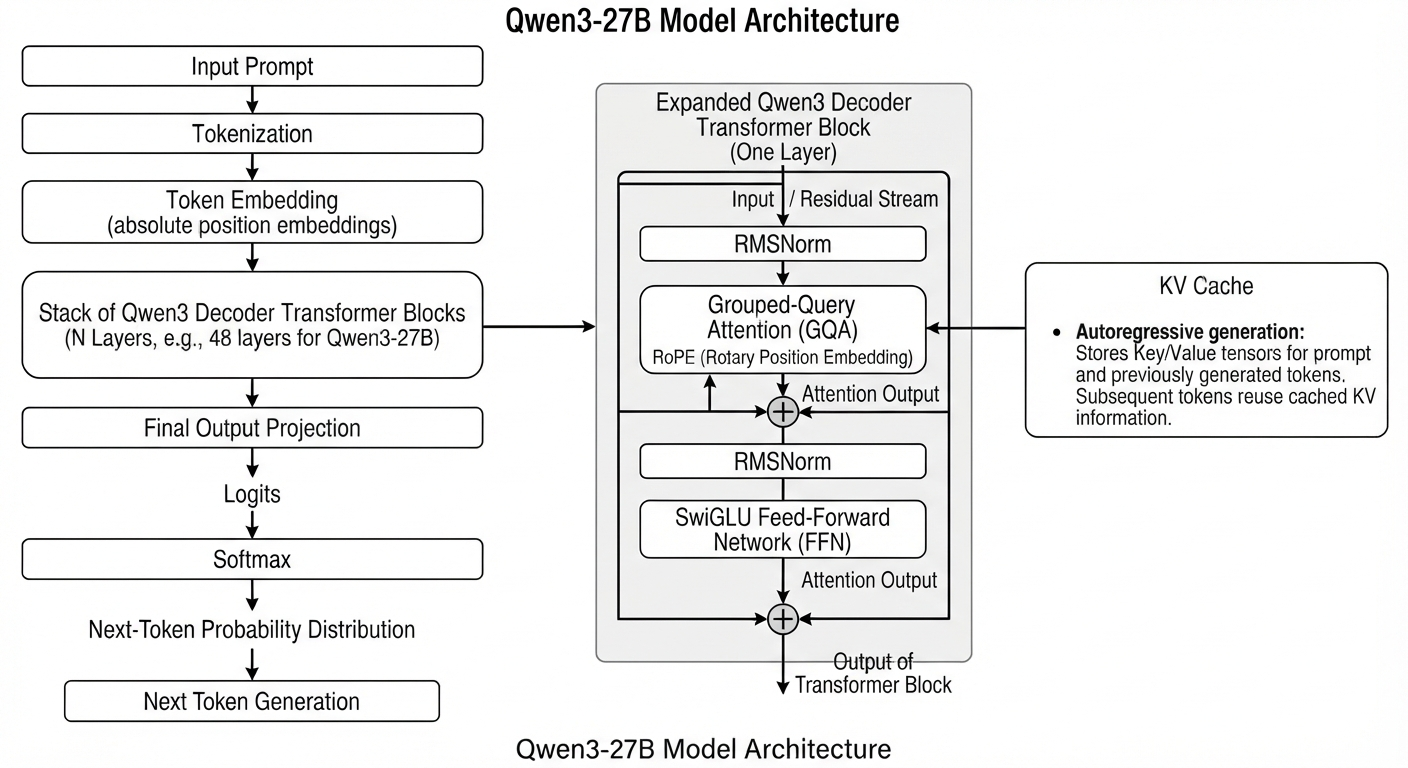
\includegraphics[width=0.9\textwidth,height=0.82\textheight,keepaspectratio]{qwen3_architecture.png}
\caption{Qwen3-style decoder-only Transformer with GQA, RoPE, SwiGLU, and RMSNorm}
\label{fig:llm-transformer-architecture}
\end{figure}

\subsection{Agent~2 API Call and Prompt Processing}
Agent~2 calls the Groq API exactly once per tagging request (or per batch for wide schemas). The call flow is as follows.

\begin{enumerate}
  \item \textbf{Prompt construction.} \texttt{\_build\_llm\_prompt} assembles a \emph{system} message that specifies the required JSON schema format and valid tag values, and a \emph{user} message containing, for each column: the column name, the heuristically inferred type, the missing-value rate, and the first three sample values. This minimal context keeps the prompt under a few hundred tokens regardless of table size.
  \item \textbf{API request.} The Groq Python client sends a \texttt{chat.completions.create} request with \texttt{model="qwen/qwen3.6-27b"} and \texttt{temperature=0.1}, \texttt{reasoning\_effort="none"}. A temperature close to zero makes the softmax distribution (Equation~\ref{eq:softmax}) sharply peaked, so the model consistently selects the highest-probability token rather than sampling freely. This near-determinism is important because the output must be strictly parseable JSON.
  \item \textbf{Prompt processing.} On Groq's LPU cluster the prompt tokens are tokenized and embedded (Equation~\ref{eq:embed}), then passed through the decoder blocks of Qwen3-27B. Inside each block, GQA (Equation~\ref{eq:gqa}) computes position-aware attention using RoPE (Equation~\ref{eq:rope}), and the SwiGLU FFN (Equation~\ref{eq:swiglu}) applies non-linear gating. RMSNorm (Equation~\ref{eq:rmsnorm}) stabilizes each sub-layer. The final block projects to logits over the vocabulary and applies softmax to produce the next-token distribution.
  \item \textbf{KV cache and autoregressive generation.} After the prompt is processed, the key and value tensors for every prompt token are cached. Each subsequent output token is generated by running only the new token through the network, attending to the cached values. This KV-cache mechanism makes generation fast even for long prompts.
  \item \textbf{Gemini failover.} If the Groq call fails or returns an unparseable response, the system automatically falls back to Google Gemini (\texttt{gemini-flash-latest}, then \texttt{gemini-3.6-flash}, \texttt{gemini-3.5-flash}, \texttt{gemini-2.5-flash}) through \texttt{\_call\_gemini\_json\_with\_failover}. If all LLM providers fail, \texttt{\_fallback\_blueprint} constructs a conservative schema from the locally sniffed types, ensuring the pipeline always has a usable blueprint.
  \item \textbf{Response parsing.} The generated text is returned in the API response body. \texttt{\_parse\_schema\_blueprint\_response} extracts valid JSON from raw or code-fenced output; as a last resort it locates the outermost \texttt{\{...\}} span so that a stray formatting character does not discard an otherwise correct schema. If parsing fails after retries, \texttt{\_fallback\_blueprint} constructs a conservative schema from the locally sniffed types, ensuring the pipeline always has a usable blueprint.
\end{enumerate}

This design keeps Agent~2 loosely coupled to the model provider: the entire LLM interaction is isolated inside a few functions (\texttt{\_build\_llm\_prompt}, the Groq/Gemini client calls, and \texttt{\_parse\_schema\_blueprint\_response}), so the backend can be swapped for another OpenAI-compatible endpoint without touching the rest of the pipeline.

\chapter{SYSTEM ARCHITECTURE AND METHODOLOGY}

\section{Overall Pipeline}
The backend pipeline is built as a directed sequence of agents using LangGraph's \texttt{StateGraph}. Each agent consumes the current \texttt{GraphState}, writes its own outputs back into the shared state, and passes the result to the next step. This keeps the workflow clear and makes debugging easier. The pipeline is orchestrated with conditional edges that gate the flow based on errors and validation results.

\begin{figure}[H]
\centering
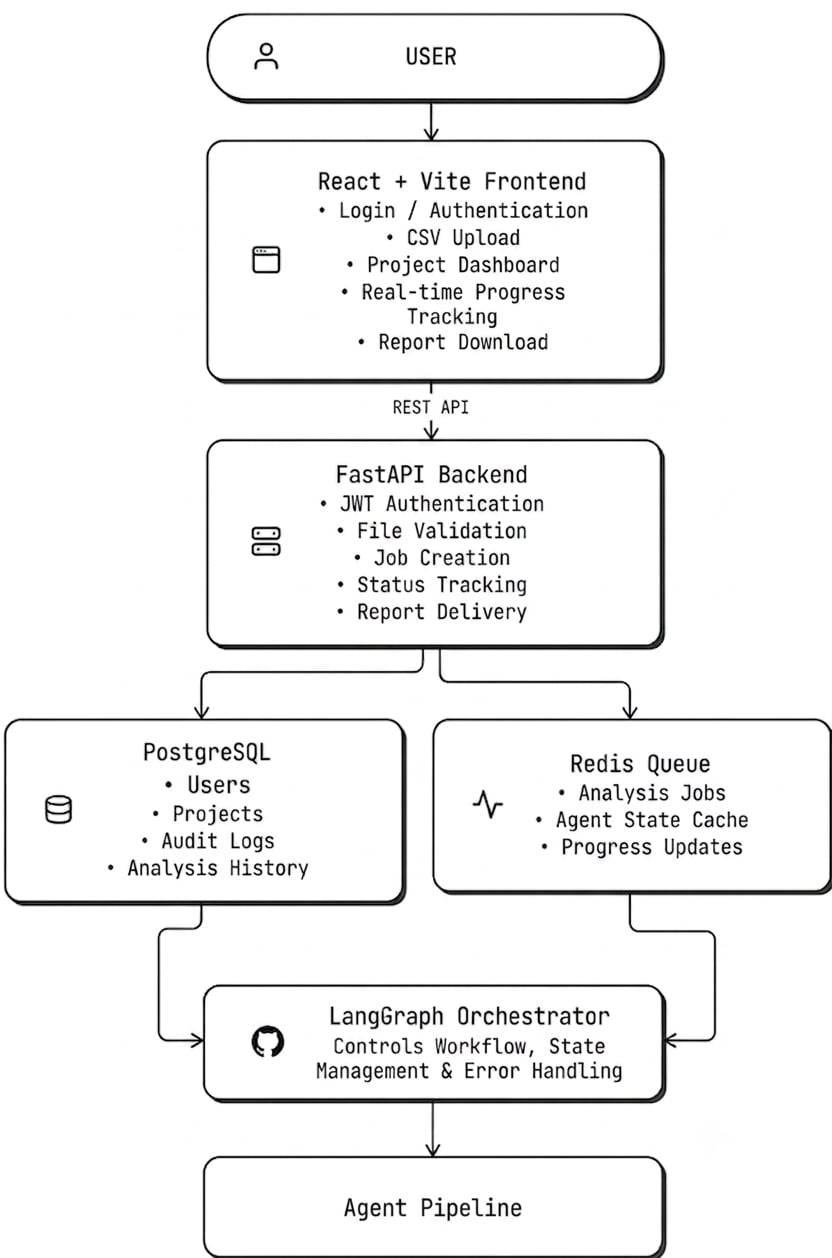
\includegraphics[width=0.82\textwidth,height=0.62\textheight,keepaspectratio]{last.jpg}
\caption{System architecture and agent flow (six-agent pipeline)}
\label{fig:system-architecture}
\end{figure}

\begin{figure}[H]
\centering
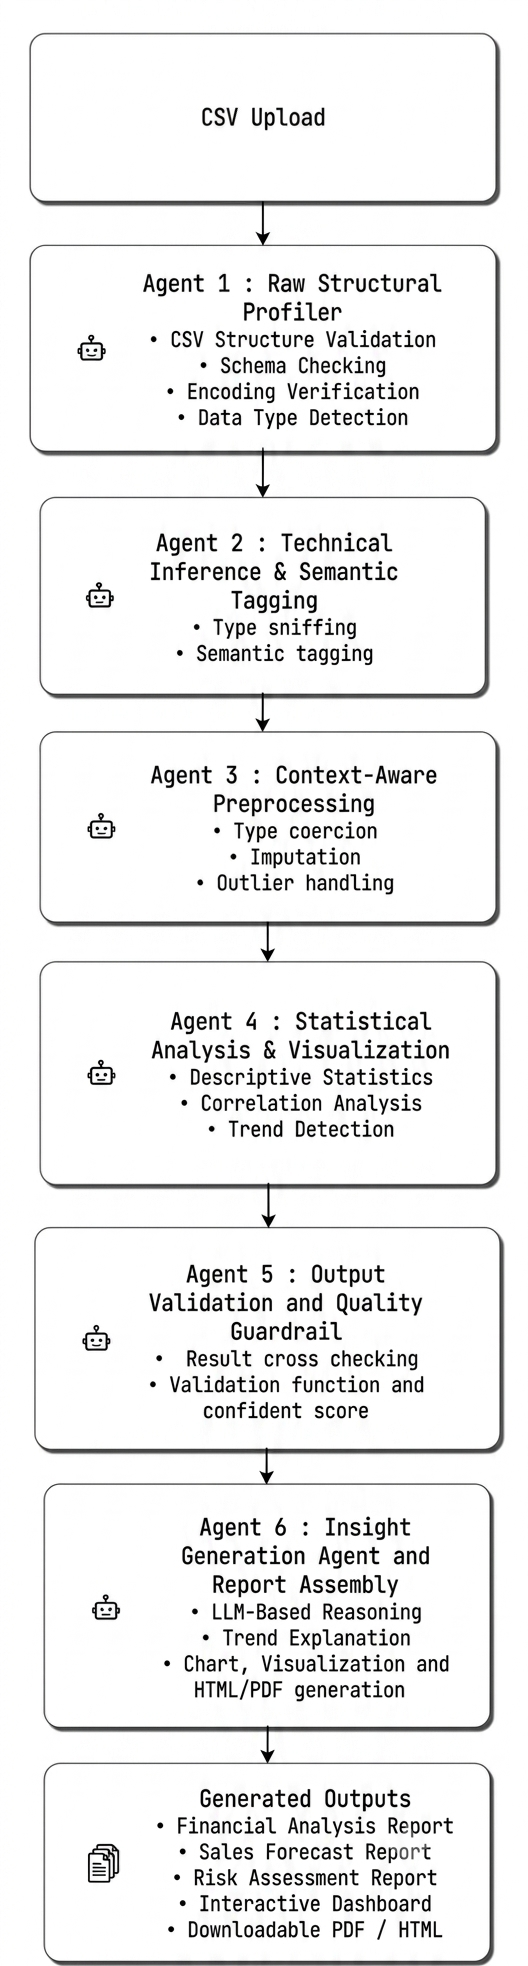
\includegraphics[width=0.9\textwidth,height=0.82\textheight,keepaspectratio]{second2.png}
\caption{LangGraph workflow showing conditional routing and Agent 5 gate}
\label{fig:agent-workflow}
\end{figure}

\section{Shared State Design}
The shared state (\texttt{GraphState}) contains the input path, the raw profile, the semantic blueprint, the cleaned dataset, the scaling parameters, the preprocessing log, the quality score, the statistics, the chart paths, an error list, and reliability metadata. This design allows each agent to focus on one responsibility while still keeping the whole workflow connected. The state also carries validation results, insight facts, narrative, and the final report path.

The state also carries reliability metadata. Each stage contributes a confidence score and evidence list, which helps the system decide whether a later stage should proceed. That is useful in the report because it shows that the project is not just generating outputs, but also measuring the reliability of those outputs.

\section{LangGraph Orchestration and Conditional Routing}
The pipeline is built with \texttt{langgraph.graph.StateGraph(GraphState)}. Nodes are \texttt{agent1..agent6}, with entry point \texttt{agent1}. Conditional edges gate the flow:

\begin{itemize}
	\item After \textbf{Agent 1}: end if any error containing "Agent1" or no \texttt{raw\_profile}, else $\rightarrow$ Agent 2.
	\item After \textbf{Agent 2}: end if "Agent2" error or no \texttt{schema\_blueprint}, else $\rightarrow$ Agent 3.
	\item After \textbf{Agent 3}: end only if \texttt{cleaned\_df is None} (non-fatal "Agent3:" warnings do not abort), else $\rightarrow$ Agent 4.
	\item After \textbf{Agent 4}: end if "Agent4" error, else $\rightarrow$ Agent 5.
	\item After \textbf{Agent 5}: end if "Agent5" error \textbf{or} \texttt{validation\_report["passed"]} is falsy — i.e. Agent 5 is a hard quality gate: a failed validation stops the pipeline before reporting, else $\rightarrow$ Agent 6.
	\item \textbf{Agent 6} $\rightarrow$ END.
\end{itemize}

\section{Reliability and Confidence Propagation}
The system implements a reliability model where every stage contributes a confidence in $[0,1]$ into \texttt{reliability.stage\_confidence[stage]}. The overall confidence is the mean of stage confidences, and decision readiness is classified as \texttt{ready} ($\ge 0.85$), \texttt{needs\_review} ($\ge 0.65$), or \texttt{blocked} ($<0.65$). Evidence strings accumulate throughout the pipeline, providing transparency and auditability. The overall reliability is:
\begin{equation}
\bar c = \frac{1}{N} \sum_{i=1}^{N} c_i
\label{eq:overall-reliability}
\end{equation}
where $c_i$ is the confidence from agent $i$. This mechanism is implemented in \texttt{update\_reliability} in \texttt{backend/main.py}.

\section{Backend Architecture}
The FastAPI backend provides REST endpoints for authentication, file upload, job management, SSE progress streaming, report download, and a grounded RAG dataset chat.

\begin{figure}[H]
\centering
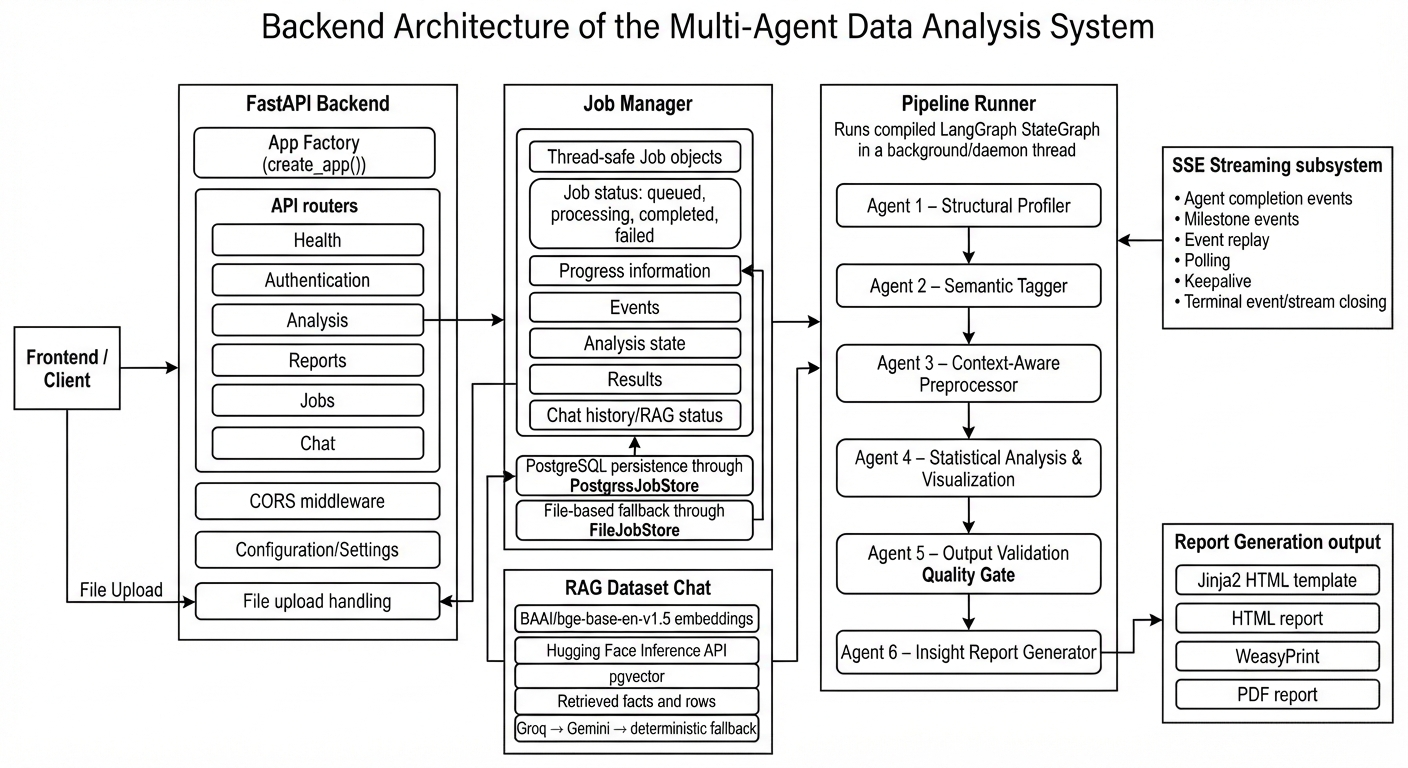
\includegraphics[width=0.9\textwidth,keepaspectratio]{backend_architecture.png}
\caption{Backend architecture: FastAPI, job manager, pipeline runner and RAG components}
\label{fig:backend-architecture}
\end{figure}

\subsection{Core Components}
\begin{itemize}
	\item \textbf{App Factory:} \texttt{create\_app()} initializes routers, CORS, and global exception handlers.
	\item \textbf{Job Manager:} Thread-safe \texttt{Job} dataclass with status, progress, events, and optional PostgreSQL (\texttt{PostgresJobStore}) or file-based (\texttt{FileJobStore}) persistence.
	\item \textbf{Pipeline Runner:} Runs compiled LangGraph in a daemon thread, emitting SSE events via \texttt{\_MilestoneEmitter} at each agent completion and key milestones.
	\item \textbf{SSE:} \texttt{/api/analyze/\{job\_id\}/stream} provides real-time progress updates with polling and keepalive.
	\item \textbf{RAG Chat:} Uses \texttt{BAAI/bge-base-en-v1.5} embeddings via Hugging Face Inference API, stores embeddings in pgvector, and grounds answers in retrieved facts and rows.
\end{itemize}

\subsection{API Endpoints}
Key endpoints are summarized in Table \ref{tab:api-endpoints}.

\begin{table}[H]
\centering
\caption{FastAPI backend endpoints}
\label{tab:api-endpoints}
\begin{tabular}{p{4cm} >{\centering\arraybackslash}p{3.5cm} p{6cm}}
\hline
Endpoint & Method & Description \\
\hline
\texttt{/api/health} & GET & Health check \\
\texttt{/api/auth/signup} & POST & User registration with PBKDF2-SHA256 hashing \\
\texttt{/api/auth/login} & POST & User login, returns JWT-style token \\
\texttt{/api/analyze} & POST & Upload CSV, start analysis job, returns job ID \\
\texttt{/api/analyze/\{id\}/stream} & GET & SSE progress stream \\
\texttt{/api/analyze/\{id\}/result} & GET & AnalysisResult (charts, stats, report path) \\
\texttt{/api/jobs} & GET & List past jobs \\
\texttt{/api/jobs/\{id\}} & GET & Job summary \\
\texttt{/api/report/\{id\}} & GET & Download PDF/HTML report \\
\texttt{/api/analyze/\{id\}/chat} & GET/POST & Dataset Q\&A with RAG \\
\hline
\end{tabular}
\end{table}

\section{Frontend Workflow}
The React 19 frontend (\texttt{frontend/AnalyzeAI/}) provides a no-code interface for uploading datasets, monitoring agent progress, viewing results, and interacting with the data via RAG chat.

\begin{itemize}
	\item \textbf{Stack:} React 19.2.7, react-router-dom 7.18.1, TailwindCSS 4.3.2, shadcn/radix-ui, framer-motion, Vite 8.1.0.
	\item \textbf{Routing:} \texttt{/} (LandingPage), \texttt{/analyze} (AnalyzePage), \texttt{/analyze/:jobId} (result view), \texttt{/history} (HistoryPage), \texttt{/login}, \texttt{/signup}, \texttt{/profile}.
	\item \textbf{Authentication:} \texttt{AuthContext} stores user in localStorage; \texttt{RequireAuth} guards protected routes.
	\item \textbf{SSE Consumption:} \texttt{subscribeToJobStream} uses \texttt{EventSource} to listen for \texttt{csv\_loaded}, \texttt{pipeline\_started}, \texttt{agent\_progress}, \texttt{charts\_generated}, \texttt{validation\_passed/failed}, \texttt{report\_generated}, and \texttt{pipeline\_finished/failed} events.
	\item \textbf{Results Display:} Displays agent progress with color coding (blue through rose), KPI cards, ECharts interactive charts (embedded JSON), and a grounded dataset chat panel.
\end{itemize}

\begin{figure}[H]
\centering
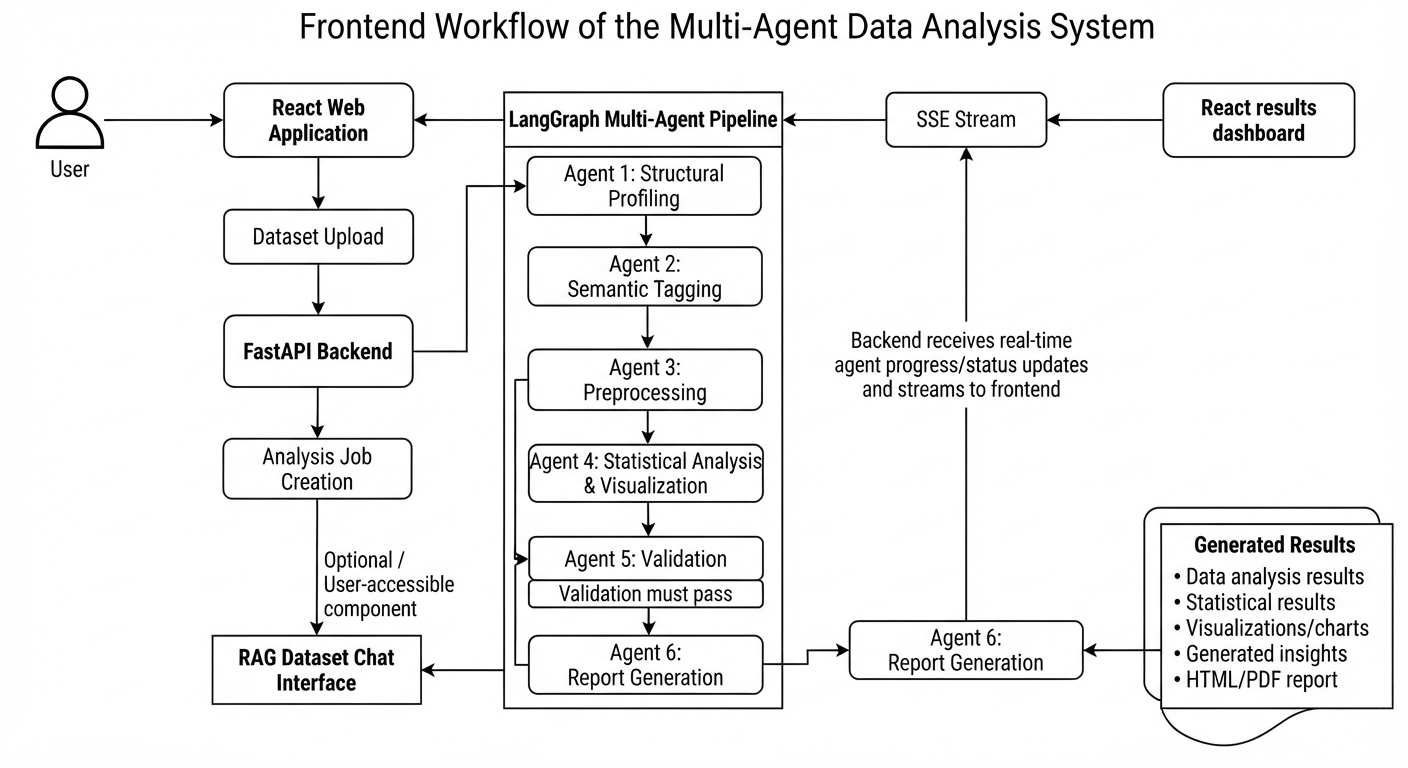
\includegraphics[width=0.8\textwidth,keepaspectratio]{frontend_workflow.png}
\caption{Frontend workflow: user upload, SSE progress, results, and RAG chat}
\label{fig:frontend-workflow-inline}
\end{figure}

\chapter{IMPLEMENTATION DETAILS}

\section{Agent 1: Structural Profiler}

\subsection{Overview and Purpose}
Agent~1 (\texttt{agent1\_structural\_profiler}) is the entry point of the pipeline. It reads the input file and records a factual description of its structure, performing no cleaning or inference so that every later stage works from an unmodified baseline.

\subsection{Inputs and Outputs}
\begin{itemize}
	\item \textbf{Inputs:} \texttt{csv\_path} from the shared \texttt{GraphState}, an optional \texttt{sheet\_name} for Excel workbooks, and the running \texttt{errors} list.
	\item \textbf{Outputs:} \texttt{raw\_profile} (per-column and dataset-level summary), the cached DataFrame \texttt{\_df\_cache}, updated \texttt{errors}, and stage \texttt{reliability} metadata.
\end{itemize}

\subsection{Processing Workflow}
The agent proceeds in four ordered stages, summarised in Figure~\ref{fig:agent1}:
\begin{enumerate}
	\item \texttt{\_load\_dataframe} selects a reader based on the file extension, routing Excel and CSV files to dedicated loaders.
	\item the chosen reader tolerates real-world messiness such as mixed delimiters and non-UTF encodings.
	\item each column is measured for type, missingness, uniqueness, and sample values.
	\item a confidence value is computed from the observed missingness and duplication.
\end{enumerate}

\begin{figure}[H]
\centering

\includegraphics[width=0.9\textwidth,height=0.82\textheight,keepaspectratio]{agent1pic.png}
\caption{Workflow of Agent~1: Structural Profiling}
\label{fig:agent1}
\end{figure}

\subsection{Key Functions}
\textbf{\texttt{\_read\_mixed\_delimiter\_csv}: resilient CSV ingestion.} Business exports are often inconsistent, mixing comma- and semicolon-separated rows under non-UTF encodings. This function first reads the text through \texttt{\_read\_csv\_lines} (trying \texttt{utf-8-sig}, \texttt{cp1252}, and \texttt{latin-1}), then detects the delimiter \emph{per line} and, when the field count does not match the header, retries with the alternate delimiter before raising an error (Figure~\ref{fig:code-agent1-csv}). It matters because a wrong delimiter would silently merge columns and corrupt every later stage. The column profiling that follows records each column's dtype, missing count and rate, unique count, and first three sample values, which Agent~2 later uses instead of the full dataset.

\begin{figure}[H]
\centering
\begin{lstlisting}[style=pystyle]
for line in lines[1:]:
    if not line.strip():
        continue

    delimiter = ";" if line.count(";") > line.count(",") else ","
    fields = next(csv.reader([line], delimiter=delimiter, quotechar='"'))

    if len(fields) != len(header):
        alternate = "," if delimiter == ";" else ";"
        alt_fields = next(csv.reader([line], delimiter=alternate, quotechar='"'))
        if len(alt_fields) == len(header):
            fields = alt_fields
        else:
            raise ValueError(
                f"Unable to parse row with {len(fields)} fields "
                f"(expected {len(header)}): {line[:120]}"
            )

    writer.writerow(fields)
\end{lstlisting}
\caption{Per-line delimiter detection and fallback in \texttt{\_read\_mixed\_delimiter\_csv} (Agent~1)}
\label{fig:code-agent1-csv}
\end{figure}

\subsection{Reliability and Pipeline Interaction}
\texttt{\_compute\_agent1\_confidence} converts the observed data health into a single confidence value that decreases with missingness and duplication:
\begin{equation}
c_1 = \text{clamp}\!\left(1 - 0.5\,\frac{m}{100} - 0.3\,\frac{d}{100},\; 0,\; 1\right)
\label{eq:agent1-conf}
\end{equation}
where $m$ is the overall missing rate and $d$ the duplicate rate as percentages. The stage is marked \texttt{ready} when $c_1 \geq 0.8$ and \texttt{needs\_review} otherwise. On success it writes \texttt{raw\_profile}, caches the DataFrame in \texttt{\_df\_cache}, and passes both to Agent~2; if loading fails, the error is recorded and the pipeline stops early. Tested on the \texttt{10000 Sales Records.csv} dataset, Agent~1 parsed the file without row loss and produced the per-column missingness and duplicate counts consumed by the later agents.

\section{Agent 2: Semantic Tagger}

\subsection{Overview and Purpose}
Agent~2 (\texttt{agent2\_semantic\_tagger}) turns the structural profile into a \texttt{schema\_blueprint}: a per-column description of the intended type, semantic role, and cleaning policy. Where Agent~1 only observed the data, Agent~2 assigns meaning to each column so that preprocessing can be driven by rules rather than guesswork. When the language model is invoked, it is called through the Groq API (\texttt{qwen/qwen3.6-27b}); the inference mechanics are described in Chapter~4 and are not repeated here.

\subsection{Inputs and Outputs}
\begin{itemize}
	\item \textbf{Inputs:} \texttt{raw\_profile} and the cached DataFrame \texttt{\_df\_cache} from Agent~1, plus the \texttt{errors} list.
	\item \textbf{Outputs:} the \texttt{schema\_blueprint} (per-column type, semantic tag, identifier flag, scaling and imputation policy, encoding strategy, and null policy) with a \texttt{\_\_metadata\_\_} block and updated \texttt{errors}.
\end{itemize}

\subsection{Processing Workflow}
The agent combines cheap local heuristics with a controlled model call. The workflow is illustrated in three stages in Figures~\ref{fig:agent2-1} to~\ref{fig:agent2-3}.

First, local type sniffing (\texttt{\_infer\_intended\_types}) assigns a provisional type to every column, and a minimal prompt containing only column metadata and three sample values is built (Figure~\ref{fig:agent2-1}).

\begin{figure}[H]
\centering
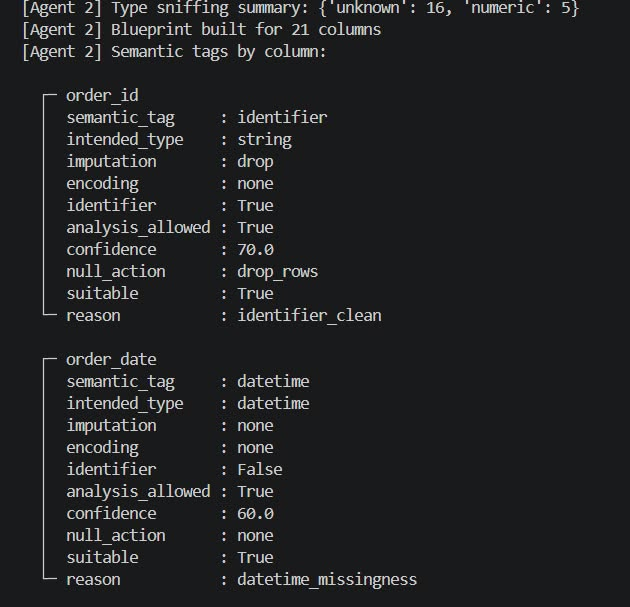
\includegraphics[width=0.9\textwidth,height=0.82\textheight,keepaspectratio]{agent21.png}
\caption{Agent~2 workflow (stage 1): local type inference and prompt construction}
\label{fig:agent2-1}
\end{figure}

Next, the model is called once for small schemas or in retry-safe batches for wide datasets and its JSON response is parsed defensively into the schema blueprint (Figure~\ref{fig:agent2-2}).

\begin{figure}[H]
\centering
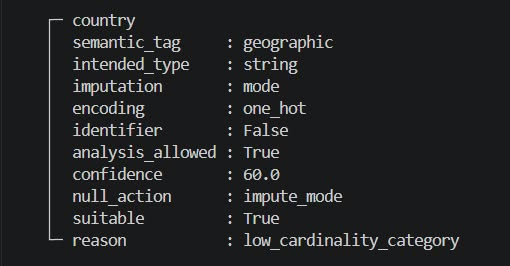
\includegraphics[width=0.9\textwidth,height=0.82\textheight,keepaspectratio]{agent22.png}
\caption{Agent~2 workflow (stage 2): batched LLM inference and schema parsing}
\label{fig:agent2-2}
\end{figure}

Finally, the blueprint is enriched: missing tags are filled, a missingness policy is applied, per-column confidence is scored, and a conservative fallback is used if the model output is unusable (Figure~\ref{fig:agent2-3}).

\begin{figure}[H]
\centering
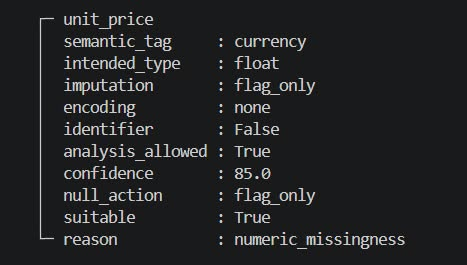
\includegraphics[width=0.9\textwidth,height=0.82\textheight,keepaspectratio]{agent23.png}
\caption{Agent~2 workflow (stage 3): enrichment, confidence scoring, and fallback}
\label{fig:agent2-3}
\end{figure}

\subsection{Key Functions}
\textbf{\texttt{\_infer\_intended\_types}} performs local type sniffing without the model, using the Pandas dtype and an 80\% parseability threshold for object columns; its result seeds both the prompt and the fallback, so every column has a defensible type even when the LLM is unavailable. \textbf{\texttt{\_build\_llm\_prompt}} sends only column metadata and three samples rather than the full table, and a fixed system prompt requires strictly valid JSON at a low temperature (0.1). For wide schemas, \textbf{\texttt{\_call\_llm\_for\_schema\_blueprint\_with\_retry}} splits columns into batches and, if a truncated response fails to parse, recursively halves the batch and merges the results, which lets the agent tag very wide datasets reliably. \textbf{\texttt{\_parse\_schema\_blueprint\_response}} accepts raw or fenced JSON and, as a last resort, extracts the outermost \texttt{\{...\}} span, so a single formatting quirk does not discard a valid schema. \textbf{\texttt{\_call\_gemini\_json\_with\_failover}} iterates through Gemini model candidates if the Groq call fails.

\subsection{Reliability and Pipeline Interaction}
After tagging, missing \texttt{semantic\_tag} values are filled and each column receives a \texttt{null\_policy} and \texttt{encoding\_strategy}; columns whose missing rate exceeds 20\% are marked \texttt{analysis\_allowed = false} so later analysis ignores unreliable fields, and \texttt{\_calculate\_semantic\_confidence} scores each tag from 0 to 100. If the model output is invalid, \texttt{\_fallback\_blueprint} assigns conservative policies from the sniffed types. On the sample \texttt{10000 Sales Records.csv} dataset, Agent~2 tagged the five monetary columns (Unit Price, Unit Cost, Total Revenue, Total Cost, Total Profit) as currency, Units Sold as a count, Region and Country as geographic, Item Type/Sales Channel/Order Priority as categorical labels, Order Date and Ship Date as datetime, and Order ID as an identifier. Example tags: \texttt{Order ID} $\rightarrow$ identifier/conf 80; \texttt{Order Date} $\rightarrow$ datetime/conf 80; \texttt{Region} $\rightarrow$ geographic/conf 65; \texttt{Unit Price} $\rightarrow$ currency/conf 65. The resulting \texttt{schema\_blueprint} is the contract that drives every decision in Agent~3.

\section{Agent 3: Preprocessor}

\subsection{Overview and Purpose}
Agent~3 (\texttt{agent3\_preprocessor}) performs deterministic cleaning and feature construction, guided entirely by the \texttt{schema\_blueprint} from Agent~2. It is the stage that turns raw, inconsistent values into a trustworthy, analysis-ready table. Unlike Agent~2, it uses no language model at all: every transformation is a fixed, logged rule, which makes the output reproducible and auditable.

\subsection{Inputs and Outputs}
\begin{itemize}
	\item \textbf{Inputs:} the cached DataFrame \texttt{\_df\_cache}, the \texttt{schema\_blueprint}, and \texttt{raw\_profile}. The agent returns early if either the frame or the blueprint is missing.
	\item \textbf{Outputs:} \texttt{cleaned\_df}, \texttt{cleaned\_csv\_path}, \texttt{scaling\_params}, \texttt{preprocessing\_log}, \texttt{data\_quality}, a \texttt{column\_ledger}, \texttt{category\_normalization}, \texttt{rule\_manifest}, and reliability metadata.
\end{itemize}

\subsection{Profile Selection}
Before any cleaning, \texttt{\_build\_preprocessing\_config} chooses a \texttt{strict}, \texttt{balanced}, or \texttt{lenient} configuration profile. A profile pinned by the caller is always honoured; otherwise \texttt{\_detect\_dataset\_domain} inspects finance keywords and currency/percentage tags and selects \texttt{strict} for finance and sales data. Each profile fixes the currency limits, the maximum plausible tax rate, the reconciliation tolerances, and the weights used later in the quality score. The profiles are summarized in Table \ref{tab:preprocessing-profiles}.

\begin{table}[H]
\centering
\caption{Preprocessing profiles}
\label{tab:preprocessing-profiles}
\small
\setlength{\tabcolsep}{4pt}
\begin{tabular}{p{1.7cm} p{1.9cm} p{1.6cm} p{1.7cm} p{1.7cm} p{3.2cm}}
\hline
Profile & currency \_max\_abs & max \_tax\_rate & recon \_rel\_tol & recon \_abs\_tol & quality weights (null / valfail / dup) \\
\hline
strict & 1.1e9 & 0.30 & 0.01 & 0.50 & 0.55 / 0.35 / 0.10 \\
balanced & 1.0e9 & 0.40 & 0.02 & 1.0 & 0.50 / 0.40 / 0.10 \\
lenient & 1.0e10 & 0.60 & 0.05 & 2.0 & 0.40 / 0.30 / 0.30 \\
\hline
\end{tabular}
\end{table}

\subsection{Processing Workflow}
Cleaning runs as an ordered, fully logged sequence of steps; each step records its per-column null differences so the effect of every action is visible. The stages, shown in Figure~\ref{fig:agent3}, are:
\begin{enumerate}
	\item \textbf{Step 0: Deduplication} \texttt{dedup\_exact\_rows} removes exact duplicate rows, asserts the count matches Agent~1's profile, and aborts through \texttt{\_assert\_row\_survival\_or\_abort} if fewer than half the rows survive (a safeguard against accidental data loss).
	\item \textbf{Step 1: Currency cleaning} \texttt{\_clean\_currency\_values} normalises monetary text and writes a \texttt{\_parse\_failed} flag for values it cannot parse.
	\item \textbf{Step 2: Type coercion} \texttt{\_coerce\_types} casts each column to its intended type while tracking any new NaNs created by the cast.
	\item \textbf{Step 3/3b: Text standardisation and re-dedup} text columns are canonicalised, then duplicates are removed again in case canonicalisation merged rows.
	\item \textbf{Step 4: Imputation} \texttt{\_impute} fills or drops missing values according to each column's policy. Supported strategies include mean, median, mode, \texttt{unknown\_label}, forward fill, KNN imputer, iterative/multivariate imputer, \texttt{drop\_rows}, \texttt{drop\_column}, \texttt{flag\_only}, and \texttt{none}. Currency and financial columns block imputation regardless of policy. Multivariate imputer results are cached across eligible columns.
	\item \textbf{Step 5: Encoding} categorical columns are encoded for later analysis (one-hot when cardinality $\le$ 10, top-8 + "Other" bucket otherwise, ordinal when order is present).
	\item \textbf{Step 6: Outlier clipping} \texttt{\_clip\_outliers} caps extreme values using percentile bounds for skewed columns and the IQR $1.5\times$ rule otherwise.
	\item \textbf{Step 7: Scaling} \texttt{\_scale\_columns} applies Min-Max scaling while preserving raw copies.
	\item \textbf{Step 8: Date features} \texttt{\_extract\_date\_features} derives calendar features from datetime columns.
	\item \textbf{Step 9: Business metrics} \texttt{\_derive\_business\_metrics} constructs profit, margin, and related fields where the necessary columns exist. Business metrics are then reconciled with ground-truth columns via \texttt{\_reconcile\_derived\_metrics}.
\end{enumerate}

\begin{figure}[H]
\centering
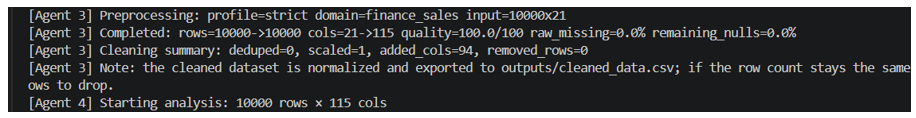
\includegraphics[width=0.9\textwidth,height=0.82\textheight,keepaspectratio]{agent3pic.png}
\caption{Workflow of Agent~3: Preprocessing Pipeline}
\label{fig:agent3}
\end{figure}

\subsection{Key Functions}

\textbf{\texttt{\_normalize\_currency\_text}: monetary parsing.} Financial exports mix symbols, currency codes, parenthetical negatives such as \texttt{(123)}, and locale-specific separators (for example the European \texttt{1.234,56} versus the US \texttt{1,234.56}). This function converts all of these to a plain numeric string so the values can be cast to \texttt{float}. Its most important part, shown in Figure~\ref{fig:code-agent3-currency}, decides which separator is the decimal point by comparing the positions of the last comma and last dot, then strips the thousands separator. Without this step, monetary columns would be read as text and every downstream financial metric would be impossible.

\begin{figure}[H]
\centering
\begin{lstlisting}[style=pystyle]
last_comma = text.rfind(",")
last_dot = text.rfind(".")

if last_comma != -1 and last_dot != -1:
    decimal_sep = "," if last_comma > last_dot else "."
    thousands_sep = "." if decimal_sep == "," else ","
    text = text.replace(thousands_sep, "")
    text = text.replace(decimal_sep, ".")
elif last_comma != -1:
    tail = text[last_comma + 1:]
    if re.fullmatch(r"\d{2}", tail):        # 1234,56 -> 1234.56
        text = text[:last_comma].replace(",", "") + "." + tail
    else:                                    # 1,234 -> 1234 (thousands)
        text = text.replace(",", "")
\end{lstlisting}
\caption{Decimal/thousands-separator resolution in \texttt{\_normalize\_currency\_text} (Agent~3)}
\label{fig:code-agent3-currency}
\end{figure}

\textbf{\texttt{\_build\_canonical\_category\_map}: fuzzy category normalisation.} This function merges similar categorical values using Levenshtein distance with guards: \texttt{FUZZY\_MATCH\_MIN\_LENGTH=6}, \texttt{FUZZY\_MATCH\_MAX\_DISTANCE=2}, first-char match, source $\le$ 5\% rows and $\le$ 1\% rare values, skip if $\le$ 3 distinct values. It logs merges and flagged ambiguous values into \texttt{category\_normalization}.

\textbf{Business metrics and reconciliation.} \texttt{\_derive\_business\_metrics} uses whole-word matching to locate revenue, cost, unit, price, discount, and budget columns, then derives: profit $= \text{rev} - \text{cost}$, margin $\% = \text{profit}/\text{rev} \times 100$, revenue per unit $= \text{rev}/\text{units}$, total revenue $= \text{price} \times \text{units}$, revenue after discount $= \text{rev} - \text{disc}$, discount $\% = \text{disc}/\text{rev} \times 100$, budget variance $= \text{rev} - \text{budget}$, budget variance $\% = \text{var}/\text{budget} \times 100$, total cost $= \text{cost} + \text{tax} + \text{shipping}$, and days to ship $= (\text{ship} - \text{order}).\text{days}$. \texttt{\_reconcile\_derived\_metrics} compares derived metrics against ground-truth columns using Pearson correlation and MAPE:
\begin{equation}
\text{MAPE} = \frac{100}{n}\sum_{i=1}^{n}\frac{|d_i - g_i|}{|g_i|}, \quad \text{diverged} \iff r < 0.99 \lor \text{MAPE} > 1.0\%
\label{eq:mape}
\end{equation}
where $d_i$ is the derived value and $g_i$ is the ground-truth column value.

\textbf{\texttt{\_impute}: imputation strategies.} Imputation strategies are summarized in Table \ref{tab:imputation-strategies}.

\begin{table}[H]
\centering
\caption{Imputation strategies supported by Agent 3}
\label{tab:imputation-strategies}
\begin{tabular}{p{3cm} p{6cm} p{3cm}}
\hline
Strategy & Description & Applicable to \\
\hline
mean & Fill with column mean & Numeric (not currency) \\
median & Fill with column median & Numeric (not currency) \\
mode & Fill with column mode & Categorical \\
unknown\_label & Fill with "Unknown" & Categorical \\
forward\_fill & Forward-fill from previous row & Any (time-series) \\
KNN & K-Nearest Neighbors imputer & Numeric (not currency) \\
iterative & Multivariate IterativeImputer & Numeric (not currency) \\
drop\_rows & Drop rows with missing values & Any (if missing rate low) \\
drop\_column & Drop entire column & Any (if missing rate high) \\
flag\_only & Create \texttt{\_is\_missing} flag, keep NaN & Any (e.g., currency) \\
none & No imputation & Any \\
\hline
\end{tabular}
\end{table}

\textbf{Other key functions.} \texttt{\_scale\_columns} applies Min-Max normalisation,
\begin{equation}
x' = \frac{x - x_{\min}}{x_{\max} - x_{\min}}
\label{eq:minmax}
\end{equation}
while keeping \texttt{\_raw} and \texttt{\_scaled} copies and storing $x_{\min}$ and $x_{\max}$ in \texttt{scaling\_params}, so the transform can be inverted later. \texttt{\_derive\_business\_metrics} uses whole-word matching (\texttt{\_find\_col}, which avoids false hits such as ``count'' matching ``Country'') to locate revenue, cost, unit, price, discount, and budget columns, then derives profit, margin, revenue per unit, discount percentage, and budget variance wherever the required columns exist, giving Agent~4 richer fields to summarise.

\subsection{Validation and Data Quality}
After the transformation steps, \texttt{\_validate\_count\_ranges} and \texttt{\_validate\_financial\_constraints} flag invalid counts and implausible tax rates into a \texttt{ColumnLedger}, and \texttt{\_compute\_enhanced\_quality\_score} combines the remaining null rate, the validation-failure rate, and the duplication rate into a single 0 to 100 \texttt{data\_quality} score. The ledger and score make the cleaning process transparent: a reviewer can see not only what the data became, but how much of it had to be corrected. The quality score is:
\begin{equation}
\begin{aligned}
Q &= w_{c}\,S_{c} + w_{v}\,S_{v} + w_{d}\,S_{d}, \\
S_c &= 100 - \text{missing\_penalty\%}, \quad S_v = 100 - \text{valfail\%}, \quad S_d = 100 - \text{dup\%}
\end{aligned}
\label{eq:quality-score}
\end{equation}
with weights per profile (Table \ref{tab:preprocessing-profiles}), and a risk penalty of $-5$ for critical issues or $-2.5$ for high issues, clamped to $[0,100]$.

\subsection{Reliability and Pipeline Interaction}
Every step appends to \texttt{preprocessing\_log} with its null differences, and the cleaned frame is exported to \texttt{outputs/cleaned\_data.csv}. Following the reliability model introduced in Equation~\ref{eq:agent1-conf}, the agent combines the quality score with the row-survival ratio into a confidence value and marks the stage \texttt{ready} or \texttt{needs\_review}. Critical failures trigger \texttt{\_early\_exit\_with\_error} so a corrupted result never propagates. On the sample dataset, Agent~3 parsed the currency fields into numeric values, extracted calendar features from the order and ship dates, one-hot encoded the region, item-type, and sales-channel columns, and derived business metrics, expanding the table from 14 to 58 columns with a data-quality score of 100.0/100. Because the sample contains no missing values, no imputation was required. The \texttt{cleaned\_df} and \texttt{scaling\_params} are the direct inputs to Agent~4.

\section{Agent 4: Statistical Analysis}

\subsection{Overview and Purpose}
Agent~4 (\texttt{agent4\_analysis}) turns the cleaned dataset into descriptive statistics and chart artifacts. It is the stage that produces measurable evidence about the data: summary statistics, correlations, trends, rankings, seasonality, anomalies, and regression fits, each accompanied by a saved figure. Before running, it clears previous PNGs with \texttt{\_clear\_chart\_dir} and writes every figure through \texttt{\_save} into \texttt{outputs/charts}, so each run starts from a clean, reproducible set of outputs.

\subsection{Inputs and Outputs}
\begin{itemize}
	\item \textbf{Inputs:} the \texttt{cleaned\_df} and \texttt{scaling\_params} from Agent~3 and the \texttt{schema\_blueprint}; it errors out if no cleaned frame exists.
	\item \textbf{Outputs:} a \texttt{stats} dictionary holding all numerical results, a \texttt{chart\_paths} list of saved figures, \texttt{chart\_specs}, updated \texttt{errors}, and reliability metadata.
\end{itemize}

\subsection{Processing Workflow}
The agent runs a fixed battery of analyses over the selected columns, illustrated in Figure~\ref{fig:agent4}:
\begin{enumerate}
	\item \textbf{Column selection} restricts analysis to meaningful fields, including \texttt{flag\_leakage\_columns} to exclude identifiers and leakage columns.
	\item \textbf{Descriptive statistics} and a \textbf{correlation} matrix (Pearson and Spearman) summarise each column and the relationships between them.
	\item \textbf{Growth rates} (MoM, QoQ), \textbf{rankings}, and \textbf{seasonality} describe how key measures change over time and across categories.
	\item \textbf{Anomaly detection} (skew-aware z-score, log-z, IQR 3$\times$ far-out fence) and \textbf{regression trends} highlight unusual values and directional change.
	\item \textbf{Distribution and derived-metric charts} visualise spread and the business fields created in Agent~3.
	\item \textbf{Cross-dimensional analyses} (6 types) explore interactions like discount-return-rate, category-margin-trend, etc.
	\item \textbf{Chart planning} uses signal-strength scoring (ANOVA $\eta^2$, Pareto, Cramér's V) to select and prioritize up to 10 charts.
\end{enumerate}

\begin{figure}[H]
\centering
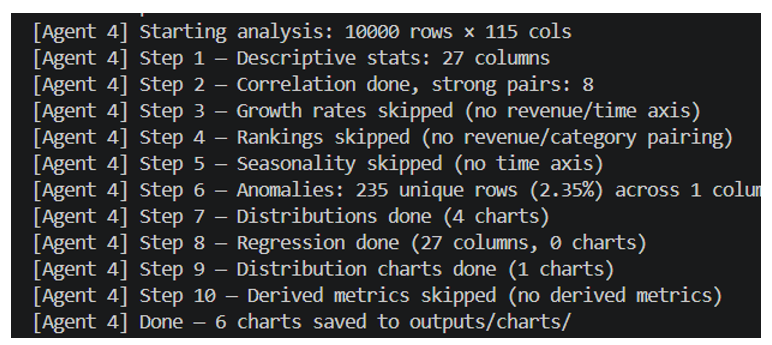
\includegraphics[width=0.9\textwidth,height=0.82\textheight,keepaspectratio]{agent4pic.png}
\caption{Workflow of Agent~4: Statistical Analysis}
\label{fig:agent4}
\end{figure}

\subsection{Key Functions}

\textbf{Column selection.} \texttt{\_numeric\_cols} and \texttt{\_categorical\_cols} decide which columns are worth analysing, excluding validation columns (\texttt{\_parse\_failed}, \texttt{\_range\_failed}), scaling backups (\texttt{\_raw}, \texttt{\_scaled}), identifiers, datetime columns, leakage columns, and any column marked \texttt{analysis\_allowed = false}. They run at the start of almost every other function, preventing meaningless output such as correlating an ID column. \texttt{flag\_leakage\_columns} detects leakage via name patterns ({classifier, naive\_bayes, \_score, \_proba, predicted\_, id, index, clientnum, customerid, \_uuid}) and correlation signatures ($|r|>0.98$ with exactly one column AND $|r|<0.1$ with $\ge n-2$ others).

\textbf{Summarisation.} \texttt{\_descriptive\_stats} computes count, mean, median, standard deviation, variance, quartiles, skewness, and kurtosis for each numeric column, while \texttt{\_correlation} computes Pearson and Spearman matrices, renders a heatmap, and records the "strong" pairs ($|r| \geq 0.5$, labelled strong when $|r| \geq 0.7$), which points the reporting stage at the relationships most worth explaining.

\textbf{\texttt{\_detect\_anomalies}: statistical outlier flagging.} This function is skew-aware:
\begin{itemize}
	\item If $|\text{skew}| \le 1.0$: use z-score $z = \frac{x - \mu}{\sigma}$, flag $|z| > 3.5$.
	\item If $|\text{skew}| > 1.0$ and positive: use log-z on $\log(1+x)$.
	\item If heavy skew or negative values: use IQR with 3.0$\times$ far-out fence: lower $= Q_1 - 3.0 \cdot \text{IQR}$, upper $= Q_3 + 3.0 \cdot \text{IQR}$.
\end{itemize}
It reports both the per-column anomalies and the count of unique affected rows, which lets the pipeline judge how "noisy" a dataset is. Columns with too few points or zero variance are skipped so the score stays well defined. The core z-score loop is shown in Figure~\ref{fig:code-agent4-anom}.

\begin{figure}[H]
\centering
\begin{lstlisting}[style=pystyle]
for col in _numeric_cols(df, schema_blueprint):
    s = df[col].dropna()
    if len(s) < 4:
        continue
    mean, std = s.mean(), s.std()
    if std == 0:
        continue
    z_scores = (df[col] - mean) / std
    anomaly_mask = z_scores.abs() > z_threshold
    anomaly_indices = df.index[anomaly_mask].tolist()
    if anomaly_indices:
        all_anomaly_indices.update(anomaly_indices)
\end{lstlisting}
\caption{$z$-score anomaly detection in \texttt{\_detect\_anomalies} (Agent~4)}
\label{fig:code-agent4-anom}
\end{figure}

\textbf{Trend and regression analysis.} \texttt{\_growth\_rates} uses a revenue column together with the \texttt{\_month}/\texttt{\_year} features from Agent~3 to plot month- and quarter-over-quarter change:
\begin{equation}
g_t = \frac{v_t - v_{t-1}}{v_{t-1}} \times 100
\label{eq:growth}
\end{equation}
\texttt{\_top\_bottom\_rankings} ranks revenue across up to three categories, and \texttt{\_seasonality} plots monthly averages with the best and worst months. \texttt{\_regression\_trends} fits an ordinary least-squares line on the \texttt{\_month} axis with \texttt{scipy.stats.linregress}:
\begin{equation}
\hat{y} = \beta_1 x + \beta_0, \quad R^2 = r^2, \quad \text{significant iff } p < 0.05
\label{eq:ols}
\end{equation}
recording slope, intercept, $R^2$, $p$-value, and whether the trend is significant ($p < 0.05$). Together these functions convert the cleaned table into the directional insights a human analyst would look for.

\textbf{Chart planning and cross-dimensional analysis.} \texttt{chart\_planner.py} scores chart candidates using:
\begin{itemize}
	\item ANOVA $\eta^2 = \frac{SS_{between}}{SS_{total}}$, skip if $<0.08$.
	\item Pareto concentration $=0.6 \cdot \text{top1\%} + 0.4 \cdot \text{top3\%}$, skip if $<30$.
	\item Distribution: $|\text{skew}| + \text{outliers}$.
	\item Trend: $R^2 \cdot 100$.
	\item Seasonality: coefficient of variation.
	\item Scatter: $|r| \cdot 100$.
	\item Cramér's V: $V = \sqrt{\frac{\chi^2}{n \min(r-1,c-1)}}$.
\end{itemize}
Charts are deduplicated, sorted by priority, capped at 10, and grouped into sections (what\_matters, shape, direction, relationships, watchlist). Cross-dimensional analyses include: discount-return-rate, category-margin-trend, rep-discount-margin, segment-order-value, region-shipping-cost, shipping-lead-time.

\subsection{Reliability and Pipeline Interaction}
The agent writes the \texttt{stats} dictionary and \texttt{chart\_paths}, updates \texttt{errors}, and records reliability (0.9 when statistics were produced, otherwise 0.4) using the same \texttt{update\_reliability} mechanism described for Agent~1. On the sample dataset, Agent~4 produced descriptive statistics for 22 numeric columns, a correlation heatmap that revealed a very strong positive relationship between Unit Price and Unit Cost ($r=0.99$), and regional and item-type revenue rankings, seasonality, and derived-metric charts (16 charts in total). These statistics and charts form the evidence base that the validation and reporting stages consume.

\section{Agent 5: Output Validation \& Trust Gate}

\subsection{Overview and Purpose}
Agent~5 (\texttt{agent5\_output\_validator}) is the quality gate that ensures only trustworthy outputs proceed to report generation. It performs deterministic contract checks and a Cohen's kappa agreement test between the LLM's semantic tags and heuristic type sniffing, providing a ground-truth-free measure of tag reliability.

\subsection{Inputs and Outputs}
\begin{itemize}
	\item \textbf{Inputs:} \texttt{cleaned\_df}, \texttt{schema\_blueprint}, \texttt{stats}, \texttt{chart\_paths}, \texttt{raw\_profile}, \texttt{preprocessing\_log}, \texttt{category\_normalization}, \texttt{column\_ledger}, \texttt{rule\_manifest}.
	\item \textbf{Outputs:} \texttt{validation\_report} with \texttt{passed} (bool), \texttt{score}, \texttt{checks} (pass/warn/fail per check), \texttt{flagged\_issues}, \texttt{cohen\_kappa}, and updated \texttt{reliability}.
\end{itemize}

\subsection{Processing Workflow}
The agent proceeds in two tiers:

\subsubsection{Tier 1: Deterministic Contract Checks}
These checks are hard rules with no LLM involvement:
\begin{itemize}
	\item \textbf{Row reconciliation:} \texttt{row\_accounting} counts (raw rows, cleaned rows, dropped rows) must match.
	\item \textbf{Schema consistency:} \texttt{cleaned\_df} columns must align with \texttt{schema\_blueprint}.
	\item \textbf{Quality score:} \texttt{data\_quality} must be in $[0,100]$.
	\item \textbf{Stats numeric sanity:} Descriptive statistics must be finite; correlations in $[-1,1]$.
	\item \textbf{Chart artifact integrity:} Chart files must exist and be non-empty.
	\item \textbf{Business-rule validation:} Worst failure $\le$ \texttt{MAX\_VALIDATION\_FAIL\_PCT} = 15\%.
	\item \textbf{Category normalization safety:} Reject merges changing $>5\%$ rows or merging two frequent values.
	\item \textbf{Trend sample sufficiency:} Significant trends need $n \ge$ \texttt{MIN\_TREND\_SAMPLE\_SIZE} = 10.
\end{itemize}

\subsubsection{Tier 2: Cohen's Kappa}
\texttt{\_cohen\_kappa\_score} computes agreement between Agent~2's LLM \texttt{intended\_type} and the heuristic sniffer, coarsened to \{numeric, datetime, boolean, string\}. Cohen's kappa is:
\begin{equation}
\kappa = \frac{p_o - p_e}{1 - p_e}, \quad p_o = \text{observed agreement}, \quad p_e = \sum_{k} \hat p^A_k \hat p^B_k
\label{eq:cohen-kappa}
\end{equation}
where $\hat p^A_k$ and $\hat p^B_k$ are the proportions of each category assigned by raters A and B. The threshold is \texttt{MIN\_ACCEPTABLE\_KAPPA} = 0.4 ("fair", Landis \& Koch \cite{landis1977}).

\subsection{Scoring and Gating}
The overall validation score is:
\begin{equation}
\text{VS} = 100 \cdot \frac{\text{passed} + 0.5 \cdot \text{warned}}{\text{total}}
\label{eq:validation-score}
\end{equation}
The pipeline passes (\texttt{passed = True}) iff \texttt{failed\_checks == 0}. A failed validation stops the pipeline before Agent~6, ensuring that unreliable outputs never reach the report.

\begin{figure}[H]
\centering
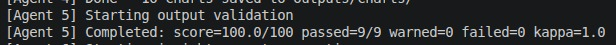
\includegraphics[width=0.9\textwidth,height=0.82\textheight,keepaspectratio]{agent5pic.png}
\caption{Agent~5 output validation implementation: Tier-1 contract checks and Cohen's kappa gate}
\label{fig:agent5-validation}
\end{figure}

\section{Agent 6: Insight Report Generator}

\subsection{Overview and Purpose}
Agent~6 (\texttt{agent6\_insight\_report\_generator}) synthesizes the validated statistics, charts, and facts into a comprehensive HTML/PDF report. It combines deterministic fact extraction with LLM-generated narrative, claim grounding, and a final hybrid composition that prioritizes verified content.

\subsection{Inputs and Outputs}
\begin{itemize}
	\item \textbf{Inputs:} \texttt{cleaned\_df}, \texttt{schema\_blueprint}, \texttt{stats}, \texttt{chart\_paths}, \texttt{chart\_specs}, \texttt{validation\_report}, \texttt{preprocessing\_log}, \texttt{category\_normalization}, \texttt{reliability}, \texttt{run\_id}.
	\item \textbf{Outputs:} \texttt{insight\_facts} (deterministic facts), \texttt{insight\_narrative} (hybrid narrative), \texttt{report\_path} (PDF/HTML), updated \texttt{reliability}.
\end{itemize}

\subsection{Processing Workflow}
The agent proceeds in seven stages:

\subsubsection{1. Deterministic Fact Extraction}
\texttt{\_extract\_insight\_facts} extracts verifiable facts from the state without using the LLM:
\begin{itemize}
	\item Dataset shape and shape-change transparency (why cleaned cols/rows differ: one-hot/ordinal/derived/date-feature/audit-trail/validation-flag).
	\item Quality facts (data\_quality, missing rates, validation score).
	\item Per-column missing-value actions reconciled against reality.
	\item Top correlations (excluding leakage/formulaic).
	\item Growth rates, rankings, profit breakdown, cross-dimensional findings.
	\item Category normalisation merges and flagged values.
	\item Anomalies (per-column and unique rows).
	\item Significant trends (OLS, $R^2$, p-value).
	\item Validation facts (Cohen's kappa, checks).
	\item Reliability (stage confidences, overall, decision\_readiness).
	\item Chart summaries.
\end{itemize}

\subsubsection{2. LLM Narrative Generation}
\texttt{\_call\_llm\_for\_narrative} calls Groq (\texttt{qwen/qwen3.6-27b}) with a strict system prompt that forbids hallucination and requires using only provided facts. It returns a JSON with: \texttt{executive\_summary}, \texttt{key\_findings}, \texttt{story} (what\_happened/why/next), \texttt{chart\_captions}, \texttt{glossary\_terms}, \texttt{plain\_language\_insights}, \texttt{bottom\_line}, \texttt{risks\_and\_caveats}, \texttt{recommendations}. Prompt facts are compacted to stay under \texttt{MAX\_NARRATIVE\_PROMPT\_CHARS}=7000. If Groq fails, the system falls back to Gemini (with the same failover chain) and finally to a deterministic fallback.

\subsubsection{3. Claim Grounding}
\texttt{\_check\_narrative\_grounding} verifies that every number in the narrative matches a computed fact within tolerance:
\begin{equation}
\text{grounded} \iff |c - k| \le \max(1.0, 0.05 \cdot |k|)
\label{eq:claim-grounding}
\end{equation}
for some known fact $k$. The grounding confidence is:
\begin{equation}
\text{conf} = \frac{\text{grounded}}{\text{checked}}
\label{eq:grounding-confidence}
\end{equation}
and the overall report confidence is $0.95$ (LLM narrative) or $0.55$ (fallback), multiplied by $(0.7 + 0.3 \cdot \text{grounding})$.

\subsubsection{4. Hybrid Composition}
\texttt{\_compose\_hybrid\_narrative} always renders the deterministic floor, then layers the LLM output only where it passes hygiene (valid story, no jargon via \texttt{\_JARGON\_PATTERNS}, known chart ids). \texttt{\_lint\_plain\_language} swaps residual jargon back to deterministic wording.

\subsubsection{5. Recommendation Grounding}
\texttt{\_ground\_recommendations} ensures each recommendation anchors to a reported finding and traceable money figures.

\subsubsection{6. Table-Cell and Raw-Column Guards}
\texttt{\_validate\_no\_empty\_required\_cells} and \texttt{\_validate\_raw\_column\_count} fail loudly on empty required cells or shape drift.

\subsubsection{7. Rendering}
The report is rendered using Jinja2 (\texttt{insight\_report.html.jinja}) with base64-embedded PNGs and embedded ECharts option JSON for interactive charts. KPI hero cards and narrative sections are grouped. \texttt{WeasyPrint} converts HTML to PDF, with a graceful fallback to HTML if PDF libraries are unavailable. Output is saved to \texttt{outputs/reports/<run\_id>/insight\_report.{pdf|html}}.

\begin{figure}[H]
\centering
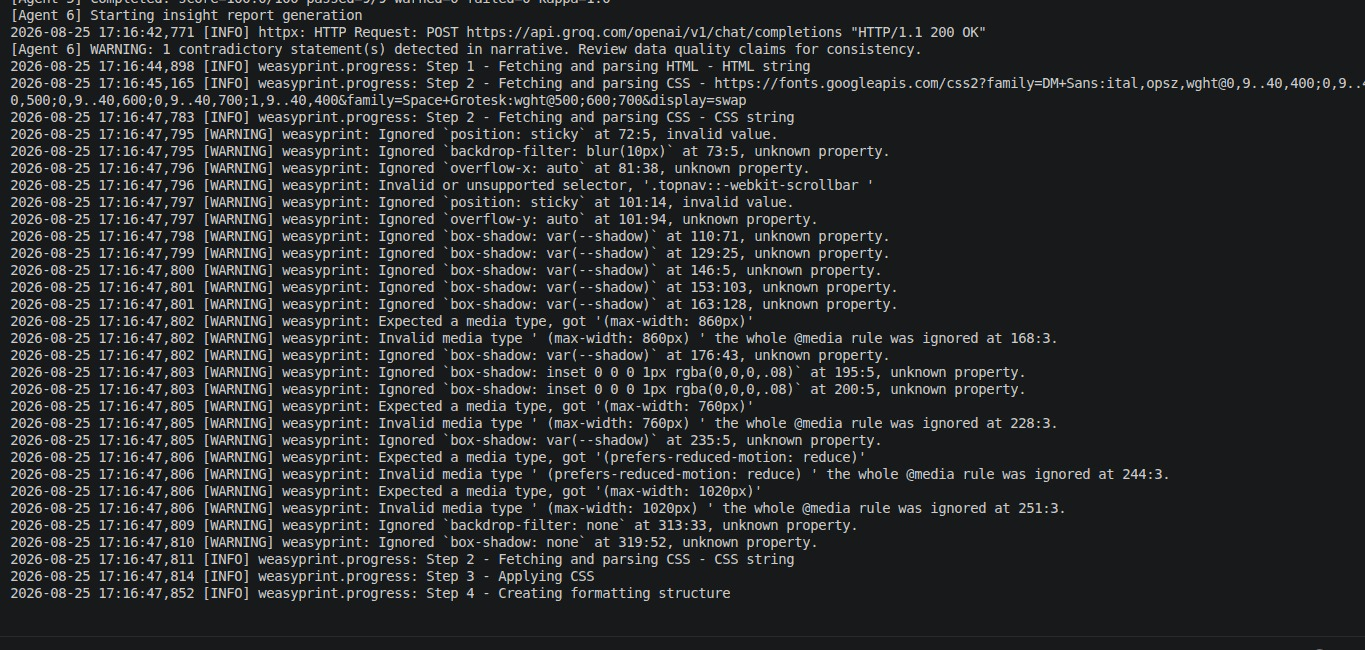
\includegraphics[width=0.9\textwidth,height=0.82\textheight,keepaspectratio]{agent6pic.png}
\caption{Agent~6 insight report generation implementation: facts $\rightarrow$ LLM narrative $\rightarrow$ hybrid+grounding $\rightarrow$ Jinja2/WeasyPrint}
\label{fig:agent6-report}
\end{figure}

\section{Backend API Implementation}

\subsection{App and Configuration}
The FastAPI app is created via \texttt{create\_app()}, which registers routers for health, auth, analysis, reports, jobs, and chat. CORS is enabled via \texttt{middleware/cors.py}. Configuration is managed by \texttt{Settings} (via \texttt{@lru\_cache}) with environment variables for uploads directory, outputs, max upload size (50 MB), allowed extensions (`.csv`), SSE poll interval (0.15s), keepalive (15s), max concurrent jobs (4), job TTL (3600s), PostgreSQL connection, RAG embedding model (\texttt{BAAI/bge-base-en-v1.5}), and Hugging Face token.

\subsection{Endpoints}
Key endpoints are summarized in Table \ref{tab:api-endpoints}. Authentication uses JWT-style tokens with PBKDF2-SHA256 password hashing (via \texttt{passlib}). User and job data are stored in PostgreSQL tables (\texttt{app\_users}, \texttt{analysis\_jobs}) with a file-based fallback (\texttt{outputs/analysis\_jobs.json}) if PostgreSQL is unavailable.

\subsection{Job Manager and Pipeline Runner}
The \texttt{JobManager} maintains thread-safe \texttt{Job} dataclasses with status (queued/processing/completed/failed), per-agent progress, append-only events for SSE, state, result, chat history, and RAG status. Jobs are persisted via \texttt{PostgresJobStore} or \texttt{FileJobStore}. The \texttt{PipelineRunner} runs the compiled LangGraph in a daemon thread, streaming values and emitting SSE events at each agent completion and key milestone.

\subsection{SSE Streaming}
Server-Sent Events are implemented in \texttt{sse.py} with format: \verb|event: <name>\n data: <json>\n\n|. Past events are replayed on connection, polling occurs every 0.15s, keepalive is sent every 15s, and the stream closes on terminal events. The stream is multi-subscriber safe.

\subsection{RAG Dataset Chat}
The RAG service uses \texttt{BAAI/bge-base-en-v1.5} embeddings via the Hugging Face Inference API when the required \texttt{DATABASE\_URL} and Hugging Face token are configured. pgvector stores embeddings for row-docs from the original uploaded CSV and fact-docs derived from the generated analysis context. During retrieval, the service retrieves top row documents (default $K=8$), top column/statistic fact documents (default $K=6$), and always includes important dataset-wide facts such as summaries, validation, correlations, rankings, anomalies, and existing charts. The chat service passes the retrieved context and recent chat history to Groq $\rightarrow$ Gemini $\rightarrow$ deterministic fallback for response generation. If the database or embedding service is unavailable, the implemented fallback answers from the deterministic summary facts rather than claiming full vector retrieval. It can optionally generate a fresh chart based on the query.

\section{Frontend Implementation}

\subsection{Stack and Structure}
The frontend (\texttt{frontend/AnalyzeAI/}) uses React 19.2.7, react-router-dom 7.18.1, TailwindCSS 4.3.2, shadcn/radix-ui, framer-motion, and Vite 8.1.0. No Redux is used; state is managed via React Context (\texttt{AuthContext}, \texttt{ThemeContext}) and per-page useState. Charts are rendered from backend ECharts JSON; there is no npm charting library.

\begin{figure}[H]
\centering
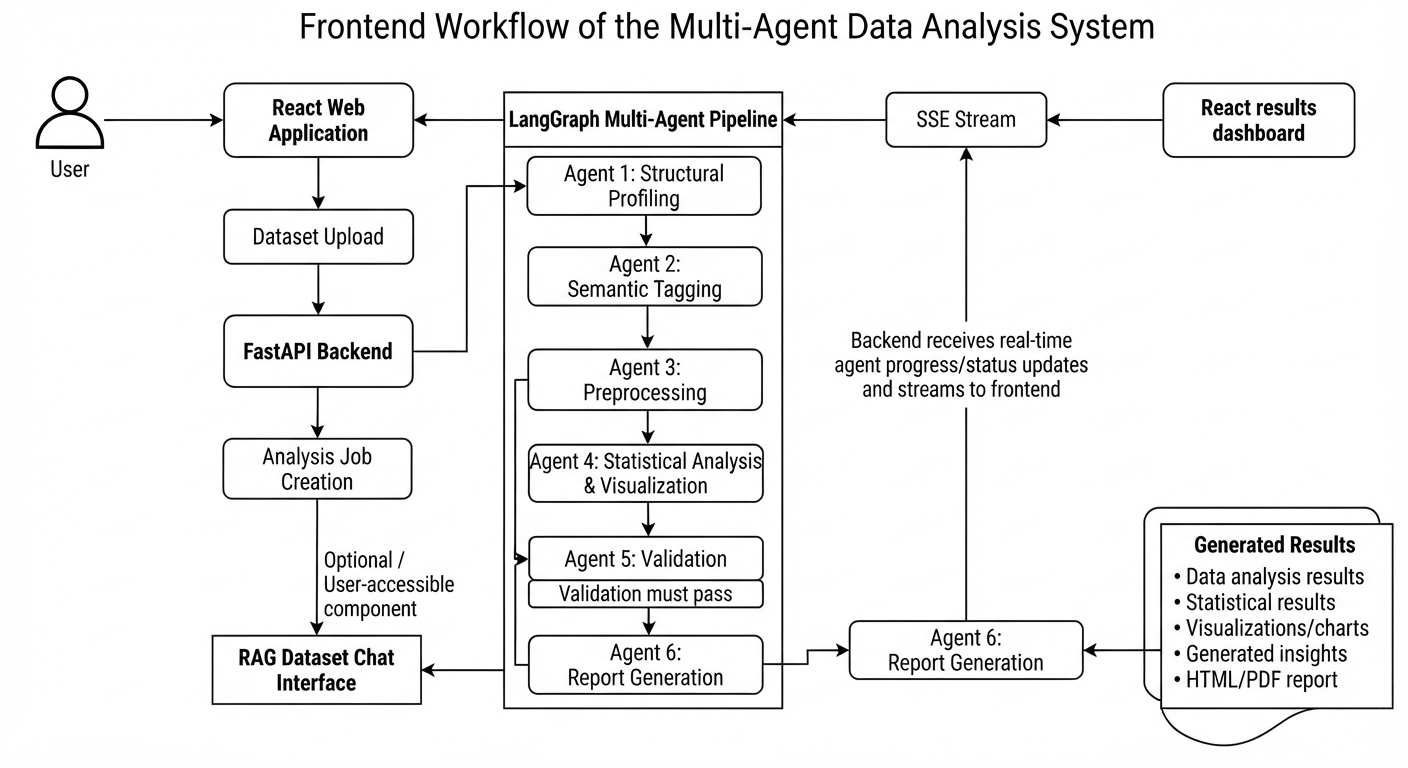
\includegraphics[width=0.9\textwidth,keepaspectratio]{frontend_workflow.png}
\caption{Frontend workflow: user upload, SSE progress, results, and RAG chat}
\label{fig:frontend-workflow-impl}
\end{figure}

\subsection{Routing and Authentication}
BrowserRouter provides routes: \texttt{/} (LandingPage), \texttt{/analyze} + \texttt{/analyze/:jobId} (AnalyzePage, wrapped in RequireAuth), \texttt{/history} (HistoryPage), \texttt{/login}, \texttt{/signup}, \texttt{/profile}. \texttt{RequireAuth} redirects to \texttt{/login} if no user is in localStorage.

\subsection{API Client and SSE}
The API client (\texttt{src/lib/api.js}) provides \texttt{analyzeCsv} (FormData upload), \texttt{subscribeToJobStream} (EventSource listening for all event types), \texttt{fetchJobResult}, \texttt{fetchJobs}, \texttt{chat}, and \texttt{reportDownloadUrl}. The EventSource listens for \texttt{csv\_loaded}, \texttt{pipeline\_started}, \texttt{agent\_progress}, \texttt{charts\_generated}, \texttt{validation\_passed/failed}, \texttt{report\_generated}, \texttt{pipeline\_finished/completed/failed}, and \texttt{error}.

\subsection{Key Components}
- \textbf{AnalyzePage:} Handles file upload, displays live agent progress with color coding (blue for Agent 1, cyan, emerald, amber, rose, violet), shows results dashboard with KPI cards, and includes \texttt{DatasetChat} for grounded Q\&A.
- \textbf{HistoryPage:} Lists past analyses with rows, cols, quality, confidence, duration.
- \textbf{AppNavbar, ThemeToggle, shadcn/radix UI primitives.}

\chapter{RESULTS AND ANALYSIS}

This chapter presents the results from a complete end-to-end run of the pipeline on the \texttt{10000 Sales Records.csv} dataset. The outputs include per-agent logs, diagnostic JSON, generated charts, and the final HTML/PDF report. All results are derived from actual executions of the implemented codebase.

\section{Pipeline Execution Summary}

A complete run on the sample dataset produces the following per-stage summary (captured from the run diagnostics):

\begin{itemize}
	\item \textbf{Agent 1:} Profiled 10000 rows $\times$ 14 columns; missing 0.0\%, duplicates 0.
	\item \textbf{Agent 2:} Type sniffing \{string:5, datetime:2, numeric:7\}; blueprint built for 14 columns.
	\item \textbf{Agent 3:} profile=strict, domain=finance\_sales, input 10000$\times$14 $\rightarrow$ cleaned 10000$\times$58, quality=100.0/100, remaining nulls 0.0\%.
	\item \textbf{Agent 4:} 22 descriptive columns, 10 strong correlation pairs, 52 anomalous rows (0.52\%), 16 charts saved.
	\item \textbf{Agent 5:} validation score 100/100, 9/9 checks passed, Cohen's kappa = 1.0.
	\item \textbf{Agent 6:} narrative source = Groq, 21/21 claims grounded, report written to \texttt{outputs/reports/<run\_id>/insight\_report.html} (HTML fallback; see below).
\end{itemize}

\section{Per-Agent Outputs}

\subsection{Agent 1: Structural Profiling}
The agent successfully loaded the CSV file, detected the correct delimiter (comma), and profiled all 14 columns. No missing values or duplicate rows were detected in this sample. The raw profile served as the baseline for all downstream stages.

\subsection{Agent 2: Semantic Tagging}
Agent 2 produced a 14-column schema blueprint (the LLM output is used when available, with a heuristic fallback). Representative tags from the sample run:
\begin{itemize}
	\item \texttt{Order ID} $\rightarrow$ identifier / conf 80
	\item \texttt{Order Date}, \texttt{Ship Date} $\rightarrow$ datetime / conf 80
	\item \texttt{Region}, \texttt{Country} $\rightarrow$ geographic / conf 65
	\item \texttt{Item Type}, \texttt{Sales Channel}, \texttt{Order Priority} $\rightarrow$ categorical label / conf 75
	\item \texttt{Units Sold} $\rightarrow$ count / conf 65
	\item \texttt{Unit Price}, \texttt{Unit Cost}, \texttt{Total Revenue}, \texttt{Total Cost}, \texttt{Total Profit} $\rightarrow$ currency / conf 65
\end{itemize}
On this run the heuristic type sniffer and the assigned intended types agreed on every column, yielding a Cohen's kappa of 1.0 (perfect agreement), later confirmed by Agent 5.

\subsection{Agent 3: Preprocessing}
Using the automatically selected \texttt{strict} profile (finance\_sales domain), the agent performed:
\begin{itemize}
	\item Currency cleaning on the five monetary columns (Unit Price, Unit Cost, Total Revenue, Total Cost, Total Profit).
	\item Type coercion of object columns to their intended types, with \texttt{format="mixed"} datetime parsing on Order Date and Ship Date.
	\item Imputation: no missing values were present, so no imputation was required.
	\item Adaptive outlier clipping on eligible numeric columns (currency/identifier columns are excluded).
	\item Min-Max scaling of eligible numeric columns, preserving \texttt{\_raw} and \texttt{\_scaled} copies.
	\item Date-feature extraction and one-hot encoding of Region, Item Type, and Sales Channel; ordinal encoding of Order Priority.
	\item Business-metric derivation with ground-truth reconciliation against the existing Total Profit column.
\end{itemize}
The cleaned dataset expanded from 14 to 58 columns due to one-hot encoding and derived features, with a data-quality score of 100.0/100 and no flagged validation issues.

\subsection{Agent 4: Statistical Analysis and Visualization}
Agent 4 produced descriptive statistics, correlations, trends, and 16 charts (a representative subset is listed in Table \ref{tab:generated-charts}). Key findings on the sample run:
\begin{itemize}
	\item \textbf{Descriptive stats:} 22 numeric columns were summarised (count, mean, median, standard deviation, variance, quartiles, skewness, kurtosis).
	\item \textbf{Correlation:} 10 pairs with $|r| \ge 0.5$ were identified. The strongest was \texttt{Unit Price} vs \texttt{Unit Cost} ($r=0.99$), followed by \texttt{Unit Price} vs \texttt{Total Cost} ($r=0.75$) and \texttt{Unit Price} vs \texttt{Total Revenue} ($r=0.73$); \texttt{Units Sold} correlated moderately with \texttt{Total Profit} ($r=0.60$) and \texttt{Total Revenue} ($r=0.52$).
	\item \textbf{Anomalies:} 52 rows (0.52\%) were flagged as statistical outliers using the skew-aware detector.
	\item \textbf{Trends:} OLS regression was fitted on the available time axis; none of the 8 candidate trends met the significance and minimum-sample thresholds on this sample, so no trend was reported as significant.
	\item \textbf{Rankings and seasonality:} Revenue and profit were ranked across Region and Item Type, and monthly/quarterly revenue and seasonality were charted.
\end{itemize}

\begin{table}[H]
\centering
\caption{Representative charts generated by Agent 4 (16 total)}
\label{tab:generated-charts}
\begin{tabular}{p{6.5cm} p{3cm} p{4cm}}
\hline
Chart Name & Type & Description \\
\hline
correlation\_heatmap.png & Heatmap & Pearson correlations among numeric columns \\
boxplot\_numeric\_cols.png & Boxplot & Spread of numeric columns \\
total\_revenue\_histogram.png & Histogram & Distribution of total revenue \\
scatter\_unit\_price\_vs\_unit\_cost.png & Scatter & Unit price vs unit cost \\
monthly\_total\_revenue\_growth.png & Line & Month-over-month revenue \\
monthly\_total\_revenue\_seasonality.png & Line & Monthly revenue seasonality \\
top\_5\_region\_total\_revenue.png & Bar & Top regions by revenue \\
top\_5\_item\_type\_total\_revenue.png & Bar & Top item types by revenue \\
top\_5\_region\_total\_profit.png & Bar & Top regions by profit \\
shipping\_lead\_time\_distribution.png & Histogram & Shipping lead-time distribution \\
\hline
\end{tabular}
\end{table}

\subsection{Agent 5: Validation}
All nine Tier-1 deterministic contract checks passed on the sample run:
\begin{itemize}
	\item Row reconciliation: raw 10000, cleaned 10000, dropped 0.
	\item Schema consistency: all 58 cleaned columns matched the blueprint.
	\item Quality score: 100.0 within $[0,100]$.
	\item Stats numeric sanity: all descriptive values finite; correlations in $[-1,1]$.
	\item Chart artifact integrity: all 16 chart files present and non-empty.
	\item Business-rule validation: worst failure 0\% $\le$ 15\%.
	\item Category normalization safety: no unsafe merges.
	\item Trend sample sufficiency: no significant trend fell below the minimum sample size.
\end{itemize}
Cohen's kappa between the assigned intended types and the heuristic sniffer was 1.0 (perfect agreement). The overall validation score was 100/100 (9/9 checks passed), so the gate passed and Agent 6 proceeded.

\begin{table}[H]
\centering
\caption{Cohen's kappa validation result for semantic tagging}
\label{tab:kappa-results}
\begin{tabular}{p{5cm} p{7cm}}
\hline
Field & Sample run value \\
\hline
Compared decisions & Agent~2 assigned intended type vs. heuristic type sniffer \\
Compared columns & 14 \\
Cohen's kappa & 1.0 \\
Disagreements & 0 \\
Acceptance threshold & \texttt{MIN\_ACCEPTABLE\_KAPPA} = 0.4 \\
Interpretation in this project & Semantic typing passed the agreement gate; this is an internal consistency check, not an external human-label accuracy score \\
\hline
\end{tabular}
\end{table}

\subsection{Agent 6: Report Generation}
The agent extracted deterministic facts, generated a narrative with Groq (Qwen3-27B), and grounded every numeric claim: 21 of 21 checked claims matched the computed facts (grounding confidence 1.0). The report includes KPI cards, the charts, a plain-language executive summary, key findings, a three-part story (what happened / why / next), recommendations, risks, and a glossary. On the test machine, WeasyPrint's native libraries were not installed, so the report was written as a self-contained HTML file (\texttt{insight\_report.html}); the same code produces a PDF when those libraries are present, demonstrating the documented graceful fallback.

\section{Performance and Reliability}

Table \ref{tab:reliability-results} shows the per-stage confidence scores and overall decision readiness recorded by the reliability mechanism on the sample run.

\begin{table}[H]
\centering
\caption{Reliability and confidence propagation (sample run)}
\label{tab:reliability-results}
\begin{tabular}{p{2.5cm} p{2.5cm} p{5.5cm} p{2.5cm}}
\hline
Stage & Confidence & Evidence & Readiness \\
\hline
Agent 1 & 1.00 & No missing values or duplicates & ready \\
Agent 2 & \textit{n/a} & LLM--heuristic agreement $\kappa=1.0$ & ready \\
Agent 3 & 1.00 & Quality = 100.0/100 & ready \\
Agent 4 & 0.90 & Statistics produced, 16 charts & ready \\
Agent 5 & 1.00 & 9/9 checks passed & ready \\
Agent 6 & 0.95 & Grounding 21/21, narrative = Groq & ready \\
\hline
Overall & 0.97 & \multicolumn{2}{p{8cm}}{Mean of the five stages reporting a numeric confidence; decision\_readiness = ready ($\ge 0.85$)} \\
\hline
\end{tabular}
\end{table}

\subsection{API Usage and Runtime Observability}
The implemented system uses external APIs in bounded locations: Agent~2 calls Groq for schema tagging with Gemini fallback; Agent~6 calls Groq for narrative generation with Gemini fallback; and the RAG chat uses Hugging Face embeddings plus Groq/Gemini/fallback answer generation when vector retrieval is configured. The code records provider/model/key-fingerprint usage for Agent~2 through the API-key usage tracker, and the persisted SSE event log records start/completion timestamps for each pipeline agent. However, the current implementation does not persist prompt tokens, completion tokens, total tokens, or per-call API response latency. Therefore, token counts and API latency values are not reported as numerical results in this project report.

Table \ref{tab:runtime-results} reports only execution times that can be derived from the saved API job events in \texttt{outputs/analysis\_jobs.json}. These are pipeline-stage wall-clock durations, not provider-level API latency measurements.

\begin{table}[H]
\centering
\caption{Pipeline runtime derived from persisted API event timestamps}
\label{tab:runtime-results}
\begin{tabular}{p{5cm} p{4cm} p{4cm}}
\hline
Stage & Duration (seconds) & Source \\
\hline
Agent 1 & 0.38 & SSE running/completed timestamps \\
Agent 2 & 4.66 & SSE running/completed timestamps \\
Agent 3 & 1.22 & SSE running/completed timestamps \\
Agent 4 & 6.72 & SSE running/completed timestamps \\
Agent 5 & 0.01 & SSE running/completed timestamps \\
Agent 6 & 2.48 & SSE running/completed timestamps \\
Total pipeline & 24.07 & \texttt{pipeline\_started} to \texttt{pipeline\_finished} \\
\hline
\end{tabular}
\end{table}

\begin{table}[H]
\centering
\caption{API and LLM metric availability in the current implementation}
\label{tab:api-observability}
\begin{tabular}{p{4cm} p{4cm} p{6cm}}
\hline
Metric & Status & Evidence / required change \\
\hline
LLM/API models used & Available & Model constants and service configuration identify Groq, Gemini, and Hugging Face embedding models \\
Number of LLM calls & Partially available & Agent~2 captures provider use; Agent~6 and chat calls are not yet persisted as a complete call count \\
Input / prompt tokens & Not recorded & Requires reading provider usage metadata after each response and storing it in the run state \\
Output / completion tokens & Not recorded & Requires provider response usage capture \\
Total tokens & Not recorded & Requires prompt and completion token capture per call \\
API response latency & Not recorded & Requires timing wrapper around Groq, Gemini, and Hugging Face calls \\
Agent execution time & Derivable & Persisted SSE timestamps record agent running/completed events \\
Total pipeline time & Derivable & Persisted \texttt{pipeline\_started} and \texttt{pipeline\_finished} events \\
Fallback calls & Partially observable & Fallback paths exist in code; exact fallback-attempt counts are not yet persisted \\
\hline
\end{tabular}
\end{table}

To measure token usage and API latency in future runs, the minimal implementation change is to add a shared API-call metrics wrapper around Groq, Gemini, and Hugging Face calls. That wrapper should record provider, model, agent, purpose, success/failure, fallback attempt, latency in milliseconds, and any available \texttt{prompt\_tokens}, \texttt{completion\_tokens}, and \texttt{total\_tokens}. The metrics should then be stored in the shared state and included in the diagnostics JSON. Until that instrumentation exists and the pipeline is rerun, this report should not claim numerical token counts or provider response latencies.

\subsection{RAG Chat Evaluation Status}
The dataset chat is implemented as a retrieval-augmented system when PostgreSQL/pgvector and the Hugging Face token are configured. The retrieval corpus contains two families of documents: row documents produced from the original uploaded CSV, and fact documents produced from the deterministic analysis result. The retriever embeds documents and user queries with \texttt{BAAI/bge-base-en-v1.5}; row documents are ranked by vector distance, while high-value fact types such as summaries, validation, correlations, rankings, anomalies, and chart references are always included so broad analytical questions remain grounded in computed results. The retrieved context and recent chat history are then passed to the LLM, and the final answer is generated through Groq, Gemini fallback, or deterministic fallback.

The implementation has functional tests for RAG triggering, context construction, retrieval branches, fallback behavior, and validated on-demand chart generation. It does not yet contain a labelled retrieval benchmark, so quantitative retrieval metrics have not been reported as achieved results. Table \ref{tab:rag-eval-status} separates what is implemented from what still requires an evaluation experiment.

\begin{table}[H]
\centering
\caption{RAG chat implementation and evaluation status}
\label{tab:rag-eval-status}
\begin{tabular}{p{4cm} p{3.2cm} p{6.2cm}}
\hline
Item & Status & Notes \\
\hline
RAG implementation & Implemented & Uses original CSV row-docs plus generated analysis fact-docs \\
Embedding model & Implemented & Hugging Face \texttt{BAAI/bge-base-en-v1.5} \\
Vector store & Implemented when configured & PostgreSQL with pgvector; fallback summary chat is used if unavailable \\
Retrieved rows & Configured & Default top-$K$ rows = 8 \\
Retrieved fact docs & Configured & Default top-$K$ column/stat facts = 6, plus always-included dataset-wide facts \\
Answer grounding & Implemented structurally & The prompt restricts answers to retrieved facts/rows; fallback uses deterministic summary facts \\
Precision@$K$ & Requires additional evaluation & Needs labelled relevant/not-relevant documents per test question \\
MRR & Requires additional evaluation & Needs the rank of the first relevant retrieved document per question \\
nDCG@$K$ & Requires additional evaluation & Needs graded relevance labels, e.g. 0/1/2 relevance levels \\
Recall@$K$ & Conditionally applicable & Valid only if the complete relevant document set is labelled over the indexed corpus \\
\hline
\end{tabular}
\end{table}

For a future quantitative RAG evaluation, a test set should be created with representative user questions, the expected relevant row/fact documents for each question, and optional graded relevance labels. Precision@$K$ should report how many retrieved documents are relevant, MRR should report how early the first relevant document appears, and nDCG@$K$ should reward highly relevant documents appearing near the top. Recall@$K$ should only be used when all relevant documents are known for each query; otherwise it would overstate what can be measured from the current sampled row index. No Precision@$K$, Recall@$K$, MRR, or nDCG@$K$ values are claimed in this report because that labelled experiment has not yet been performed.

\section{Error Analysis and Validation Discussion}

The system demonstrated robust error handling and validation. Key observations from the sample run:

\begin{itemize}
	\item \textbf{Currency parsing:} The European vs US decimal resolution (Figure~\ref{fig:code-agent3-currency}) correctly parsed the monetary columns to numeric values, including accounting negatives and mixed symbols.
	\item \textbf{Datetime coercion:} The \texttt{format="mixed"} flag in \texttt{pd.to\_datetime} avoids a class of bug in which mixed date formats are silently converted to NaT; the order and ship dates were parsed without row loss.
	\item \textbf{Outlier clipping:} Adaptive IQR/percentile clipping caps extreme values while excluding currency and identifier columns, preventing distortion of the statistics without discarding genuine business outliers.
	\item \textbf{Ground-truth reconciliation:} The reconciliation guardrail ($r \ge 0.99$, MAPE $\le$ 1\%) cross-checks each derived metric against any equivalent source column; on this sample no divergence was flagged.
	\item \textbf{Cohen's kappa:} The $\kappa=1.0$ agreement between the assigned types and the heuristic sniffer provides evidence that the semantic tagging is reliable without requiring ground-truth labels---a ground-truth-free trust signal.
	\item \textbf{Claim grounding:} All 21 numeric claims in the generated narrative were verified against the computed facts within tolerance, demonstrating effective hallucination control.
\end{itemize}

These results confirm that the multi-agent pipeline successfully processes a raw CSV file through all six stages, producing a validated, grounded, and professionally formatted analytical report with minimal human intervention.

\chapter{FUTURE ENHANCEMENT}

While the current system provides a complete end-to-end solution, several enhancements are planned for future development:

\begin{itemize}
	\item \textbf{Multi-format ingestion:} Extend support beyond CSV-primary to include Excel, JSON, Parquet, and direct database connections. An Excel loader path already exists, but JSON and Parquet are not yet implemented.
	\item \textbf{Model-agnostic provider configuration:} Allow users to configure their preferred LLM providers (Groq, Gemini, OpenAI, Anthropic, local models via Ollama) through a settings panel, making the system more flexible and cost-optimized.
	\item \textbf{More chart families:} Add Sankey diagrams, treemaps, geographic maps, and time-series decomposition plots to enrich the visual analysis.
	\item \textbf{Auth hardening:} Implement proper OAuth2/OpenID Connect with refresh tokens, role-based access control (RBAC), and multi-tenancy for organizational use.
	\item \textbf{Larger-scale evaluation:} Conduct systematic benchmarking on diverse datasets (100+ CSVs) to quantify accuracy, speed, and reliability across different domains and data quality levels.
	\item \textbf{Interactive report customization:} Allow users to select chart types, add custom metrics, and modify the narrative tone through a visual editor.
	\item \textbf{Continuous learning:} Implement feedback loops where user corrections (e.g., fixing a mis-tagged column) are stored and used to fine-tune the semantic tagging and preprocessing rules.
\end{itemize}

These enhancements will further increase the system's utility, scalability, and adoption in real-world business environments.

\chapter{CONCLUSION}

This project successfully developed and delivered a complete end-to-end multi-agent system for automated data analysis and insight generation from financial and sales CSV data. The system comprises six specialized agents (structural profiling, semantic tagging, context-aware preprocessing, statistical analysis and visualization, output validation, and hybrid report generation) orchestrated by LangGraph with conditional routing and a hard validation gate. A FastAPI backend provides secure file uploads, job management, Server-Sent Events for live progress streaming, and a grounded RAG dataset chat. A React 19 frontend offers a no-code web interface for uploading datasets, monitoring pipeline execution, viewing interactive charts, and downloading HTML/PDF reports.

The system's key strengths are its separation of concerns, auditability through logged transformations and confidence propagation, and reliability through deterministic contract checks, Cohen's kappa agreement scoring, and claim-grounding mechanisms that prevent hallucinated insights from reaching the final report. On a representative sample dataset, the pipeline processes a raw CSV file from ingestion through to a professionally formatted report (HTML, and PDF when WeasyPrint's native libraries are available) with KPI summaries, charts, plain-language findings, and actionable recommendations, all with minimal human intervention.

The project achieves its primary objectives: (1) an autonomous multi-agent system that converts raw data into professional reports without manual coding, and (2) a no-code web interface that democratizes financial analytics for small to medium businesses. The system is ready for deployment and use in real-world scenarios, with clear pathways for future enhancement.

The main contribution of this work is a practical, validated framework for agentic data analysis that combines deterministic algorithms with controlled LLM reasoning, ensuring reliability, reproducibility, and accessibility. This framework can serve as a blueprint for similar systems in education, non-profits, and commercial settings where data-driven decision-making is essential but technical expertise is limited.

\clearpage
\chapter{APPENDICES}

\section*{Appendix A: Dataset Details}
\addcontentsline{toc}{section}{Appendix A: Dataset Details}

The sample dataset used for validation and demonstration is \texttt{10000 Sales Records.csv}, available in the project repository. It contains 10,000 rows and 14 columns, representing simulated global sales transactions with the following columns:

\begin{itemize}
	\item \texttt{Region}: Geographic region (categorical, e.g. Sub-Saharan Africa, Europe, Asia).
	\item \texttt{Country}: Country of the transaction (categorical).
	\item \texttt{Item Type}: Product category (categorical, 12 distinct values).
	\item \texttt{Sales Channel}: Online or Offline (categorical).
	\item \texttt{Order Priority}: Order priority code (categorical: H, M, L, C).
	\item \texttt{Order Date}, \texttt{Ship Date}: Order and shipment dates (datetime).
	\item \texttt{Order ID}: Unique transaction identifier (integer).
	\item \texttt{Units Sold}: Quantity sold (integer count).
	\item \texttt{Unit Price}, \texttt{Unit Cost}: Per-unit price and cost (currency).
	\item \texttt{Total Revenue}, \texttt{Total Cost}, \texttt{Total Profit}: Aggregate monetary fields (currency).
\end{itemize}

The sample is clean (no missing values, no duplicates) and exercises the full pipeline: identifiers, dates, categories, and multiple monetary columns that support derived-metric reconciliation. The system itself is not tied to this dataset and accepts arbitrary tabular CSV files.

\section*{Appendix B: Cost Estimate}
\addcontentsline{toc}{section}{Appendix B: Cost Estimate}

\begin{table}[H]
\centering
\caption{Indicative project cost estimate}
\label{tab:cost-estimate-app}
\begin{tabular}{p{6cm} p{3cm} p{3cm}}
\hline
Item & Estimate & Notes \\
\hline
Development laptop and local machine & Existing & Already available for development \\
Python, FastAPI, LangGraph, plotting stack & Existing & Open-source software stack \\
React, Vite, TailwindCSS & Existing & Open-source frontend stack \\
PostgreSQL (optional) & Existing/FOSS & Free for local/cloud use \\
LLM API usage (Groq \& Gemini) & Variable & Usage-based; small per-run cost \\
Internet and miscellaneous expenses & Variable & Project maintenance cost \\
\hline
\end{tabular}
\end{table}

The cost estimate is intentionally lightweight because the project uses open-source libraries and an existing development environment. The main variable cost comes from API usage during testing and report generation. In practice, that cost can be managed by keeping the heuristic fallback path available, using the schema cache, and avoiding unnecessary repeated model calls. Agent~2 sends only column metadata and a few sample values rather than full rows, which limits prompt size by design; exact token counts are not currently persisted by the implementation.

\section*{Appendix C: Project Timeline}
\addcontentsline{toc}{section}{Appendix C: Project Timeline}

\begin{table}[H]
\centering
\caption{Project timeline summary}
\label{tab:timeline-app}
\begin{tabular}{p{5cm} p{4cm} p{3cm}}
\hline
Task & Status & Phase \\
\hline
Requirement analysis and proposal & Complete & Initial \\
Agent 1–4 implementation and integration & Complete & Development \\
Agent 5–6 implementation & Complete & Development \\
Backend API and frontend development & Complete & Development \\
Testing, evaluation, and debugging & Complete & Finalization \\
Documentation and report submission & Complete & Final \\
\hline
\end{tabular}
\end{table}

All major tasks are now complete. The project moved from proposal to a fully functional end-to-end system with a web interface, API, and six-agent pipeline. The final phase focused on integration testing, report generation, and documentation.

\begin{figure}[H]
\centering
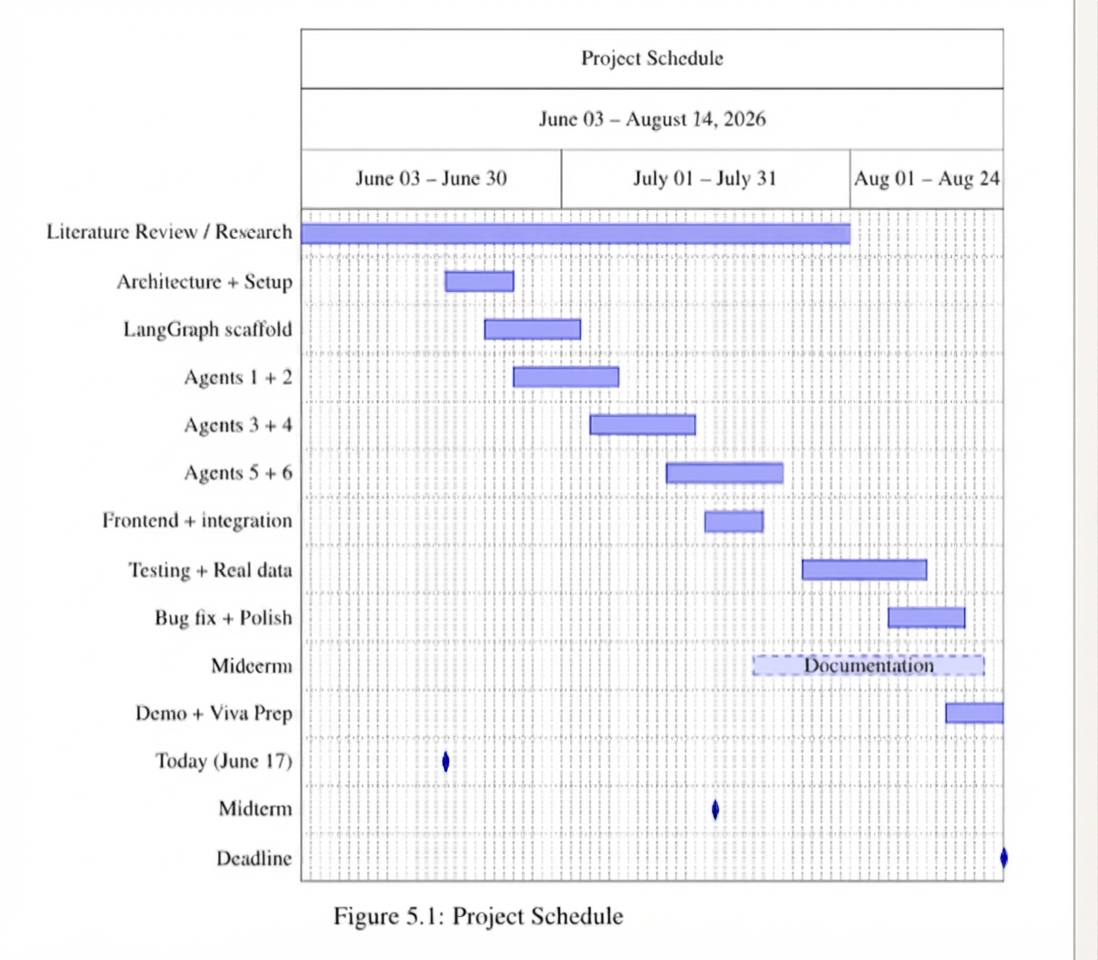
\includegraphics[width=0.9\textwidth,keepaspectratio]{project_schedule.png}
\caption{Project schedule and milestones}
\label{fig:project-schedule}
\end{figure}

\section*{Appendix D: Sample Generated Report Screenshots}
\addcontentsline{toc}{section}{Appendix D: Sample Generated Report Screenshots}

\begin{figure}[H]
\centering

\includegraphics[width=0.9\textwidth,height=0.82\textheight,keepaspectratio]{final_report.png}
\caption{Sample output: Final report demo}
\label{fig:sample-report}
\end{figure}

\begin{figure}[H]
\centering

\includegraphics[width=0.9\textwidth,height=0.82\textheight,keepaspectratio]{dashboard_screenshot.png}
\caption{Sample output: Web application results dashboard}
\label{fig:webapp-dashboard}
\end{figure}

\section*{Appendix E: Agent Run Diagnostics Excerpt}
\addcontentsline{toc}{section}{Appendix E: Agent Run Diagnostics Excerpt}

Below is a representative run summary produced by the pipeline diagnostics:

\begin{lstlisting}[style=pystyle, caption=Representative run summary from the pipeline diagnostics]
{
  "run_id": "d6816f020542",
  "raw_shape": {"rows": 10000, "cols": 14},
  "cleaned_shape": [10000, 58],
  "preprocessing_profile": "strict",
  "dataset_domain": "finance_sales",
  "data_quality": 100.0,
  "validation_passed": true,
  "validation_score": 100.0,
  "cohen_kappa": 1.0,
  "flagged_issues": 0,
  "n_charts": 16,
  "narrative_source": "groq",
  "claims_grounding": {"claims_checked": 21, "claims_grounded": 21,
                       "claims_flagged": 0, "confidence": 1.0},
  "reliability": {
    "stage_confidence": {"agent1": 1.0, "agent3": 1.0, "agent4": 0.9,
                          "agent5": 1.0, "agent6": 0.95},
    "overall_confidence": 0.97,
    "decision_readiness": "ready"
  },
  "report_path": "outputs/reports/d6816f020542/insight_report.html"
}
\end{lstlisting}

\clearpage
\phantomsection
\addcontentsline{toc}{chapter}{REFERENCES}
\begin{thebibliography}{99}

\bibitem{dwivedi2023} Y. K. Dwivedi, L. Hughes, A. M. Baabdullah, et al., ``So what if ChatGPT wrote it? Multidisciplinary perspectives on opportunities, challenges and implications of generative conversational AI for research, practice and policy,'' \textit{International Journal of Information Management}, vol. 71, 2023.

\bibitem{openai2024} OpenAI, ``GPT-4 Technical Report,'' 2024.

\bibitem{sun2024} M. Sun, R. Han, B. Jiang, H. Qi, D. Sun, Y. Yuan, and J. Huang, ``LAMBDA: A Large Model Based Data Agent,'' arXiv preprint arXiv:2407.17535, 2024.

\bibitem{liu2023chatgpt} Y. K. Liu, et al., ``Summary of ChatGPT-Related Research and Perspective Towards the Future of Large Language Models,'' arXiv:2306.07209, 2023.

\bibitem{maynez2020faithfulness} J. Maynez, S. Narayan, B. Bohnet, and R. McDonald, ``On Faithfulness and Factuality in Abstractive Summarization,'' in \textit{Proceedings of ACL}, 2020.

\bibitem{dibia2019} V. Dibia and C. Demiralp, ``Data2Vis: Automatic Generation of Data Visualizations Using Sequence-to-Sequence Recurrent Neural Networks,'' \textit{IEEE Computer Graphics and Applications}, vol. 39, no. 5, pp. 33--46, 2019.

\bibitem{hu2019} K. Hu, M. A. Bakker, S. Li, T. Kraska, and C. A. Hidalgo, ``VizML: A Machine Learning Approach to Visualization Recommendation,'' in \textit{Proceedings of the CHI Conference on Human Factors in Computing Systems}, 2019.

\bibitem{moritz2018} D. Moritz, C. Wang, G. L. Nelson, H. Lin, A. M. Smith, B. Howe, and J. Heer, ``Formalizing Visualization Design Knowledge as Constraints: Actionable and Extensible Models in Draco,'' \textit{IEEE Transactions on Visualization and Computer Graphics}, 2018.

\bibitem{luo2018} Y. Luo, X. Qin, N. Tang, and G. Li, ``DeepEye: Towards Automatic Data Visualization,'' in \textit{IEEE International Conference on Data Engineering (ICDE)}, 2018.

\bibitem{langchain2024} LangChain, ``LangGraph: A Python Library for Building Stateful, Multi-Agent Applications,'' 2024.

\bibitem{wu2023} Q. Wu, G. Bansal, J. Zhang, et al., ``AutoGen: Enabling Next-Gen LLM Applications via Multi-Agent Conversation Framework,'' 2023.

\bibitem{vaswani2017} A. Vaswani, N. Shazeer, N. Parmar, J. Uszkoreit, L. Jones, A. N. Gomez, \L. Kaiser, and I. Polosukhin, ``Attention Is All You Need,'' \textit{Advances in Neural Information Processing Systems}, vol. 30, pp. 5998--6008, 2017.

\bibitem{qwen2024} Qwen Team, ``Qwen3-27B Technical Report,'' 2024.

\bibitem{ainslie2023gqa} J. Ainslie, J. Lee-Thorp, M. de Jong, Y. Zemlyanskiy, F. Lebr\'{o}n, and S. Sanghai, ``GQA: Training Generalized Multi-Query Transformer Models from Multi-Head Checkpoints,'' in \textit{Proceedings of EMNLP}, 2023.

\bibitem{su2021rope} J. Su, Y. Lu, S. Pan, A. Murtadha, B. Wen, and Y. Liu, ``RoFormer: Enhanced Transformer with Rotary Position Embedding,'' arXiv preprint arXiv:2104.09864, 2021.

\bibitem{shazeer2020swiglu} N. Shazeer, ``GLU Variants Improve Transformer,'' arXiv preprint arXiv:2002.05202, 2020.

\bibitem{zhang2019rmsnorm} B. Zhang and R. Sennrich, ``Root Mean Square Layer Normalization,'' in \textit{Advances in Neural Information Processing Systems}, 2019.

\bibitem{landis1977} J. R. Landis and G. G. Koch, ``The Measurement of Observer Agreement for Categorical Data,'' \textit{Biometrics}, vol. 33, no. 1, pp. 159--174, 1977.

\bibitem{lewis2020rag} P. Lewis, E. Perez, A. Piktus, et al., ``Retrieval-Augmented Generation for Knowledge-Intensive NLP Tasks,'' in \textit{Advances in Neural Information Processing Systems}, 2020.

\end{thebibliography}

\end{document}